\graphicspath{ {./img/TheFEM/} }
\chapter{The Finite Element Method}
\section{Boundary value problems}
In this section we will define a general initial boundary value problem (I-BVP). In the first part we will introduce the differential formulation given in terms of a set of governing equations and properly specified boundary conditions. The resulting equations are obtained after using a generalized balance law. Following this classical and well known approach we formally re-state these equations in the so-called strong form. Subsequently we re-write and prove an equivalent form of the balance law in the form of an integral representation highly friendly for a numerical solution. Since in the integral description of the problem the order of the derivatives in the field functions decreases by one, the resulting statement is called a weak formulation. 
%%
\subsection{Differential formulation-Generalized balance law}
Let $ds$ be a differential surface element; $\dd{V}$ a differential volume element; $u(\vb{x},t)$ a scalar (or vector) function of space and time.
The flux or rate of flow of the quantity $u(\vb x, t)$ through $\dd{S}$ at time $t$ is defined like
\[p(\vb x)\grad u \cdot \hat n \dd{S} \enspace ,\]
where $p(\vb x)$ is a positive function, assumed known and time independent. Similarly, the time rate of change of $u(\vb x, t)$ in an element $\dd{V}$ is given by
\[\rho (\vb x)\pdv{u}{t} \dd{V} \enspace ,\]
where once again $\rho (\vb x)$ is a known, given, time independent positive function. Additional effects occurring in the element $\dd{V}$ at the time time can be expressed like
\[H(\vb x, t)\dd{V} \equiv  - q(\vb x)u(\vb x, t) + \hat F(\vb x,t)\]
where $\hat F(\vb x, t) = \rho (\vb x)F(\vb x, t)$. In the above the term $q u$ represent internal effects due to changes proportional to $u$ while $\hat F(\vb x, t)$ are other external influences in the medium.

Balancing the internal and external changes yields
\[\int\limits_V \rho (\vb x)\pdv{u}{t}\dd{V} = \int\limits_S p(\vb x)\vb \grad u \cdot \hat n\dd{S}  + \int\limits_V H(\vb x, t)\dd{V} \enspace ,\]
or equivalently
\[\int\limits_V \rho (\vb x)\pdv{u}{t}\dd{V} = \int\limits_S p(\vb x)\vb \grad u \cdot \hat n\dd{S}   - \int\limits_V q(\vb x)u(\vb x, t)\dd{V}  + \int\limits_V \rho (\vb x)F(\vb x, t)\dd{V} \enspace .\]

Using the divergence theorem as
\[\int\limits_S p(\vb x) \grad u \cdot \hat n \dd{S}  = \int\limits_V \vb \div  (p\vb \grad u)\dd{V}\]
yields after substitution
\[\int\limits_V \left[\rho (\vb x)\pdv{u}{t} - \div (p(\vb x)\grad u) + q(\vb x)u(\vb x, t) - \rho (\vb x)F(\vb x, t)\right]\dd{V}  = 0\]
Assuming a continuous integrand, the arbitrariness of $V$ implies
\[\rho (\vb x)\pdv{u}{t} - \div(p(\vb x)\grad u) + q(\vb x)u(\vb x, t) - \rho (\vb x)F(\vb x, t) = 0\]

Letting
\[\mathcal{L} \equiv  - \div p(\vb x)\grad + q(\vb x)\]
the generalized set of partial differential equations can be written like
\begin{equation}
\rho(\vb x) \pdv{u(\vb x, t)}{t} + \mathcal{L}u(\vb x, t) = \rho (\vb x)F(\vb x, t) \enspace .
\label{eq:GenPDE}
\end{equation}

And they are categorized as:
\begin{itemize}
    \item Hyperbolic;
    \[\rho(\vb x) \pdv[2]{u(\vb x, t)}{t} + \mathcal{L}u(\vb x,t) = 0\]

    \item Parabolic; and
    \[\rho(\vb x) \pdv{u(\vb x,t)}{t} + \mathcal{L}u(\vb x, t) = 0\]

    \item Elliptic
    \[\mathcal{L}u(\vb x, t) = \rho (\vb x)F(\vb x, t) \enspace .\]
\end{itemize}

It can be shown that $\mathcal{L}$ satisfies the \emph{symmetry} condition
\[\int\limits_V \mathcal{L}(u)v\dd{V} =  \int\limits_V \mathcal{L}(v)u \dd{V}\]
and positive definiteness \cite{book:sepulveda_fismat, book:arfken}
\[\int\limits_V \mathcal{L}(u)u\dd{V}  > 0, \quad \forall u \enspace .\]

\subsection*{Strong form}
Given $\rho(\vb x)$, $q(\vb x)$, $p(\vb x)$, $F(\vb x, t)$ and $\bar u$ find $u(\vb x , t):V \to \mathbb{R}$ such:
\[\rho(\vb x) \pdv{u}{t} - \div \left[p(\vb x) \grad u\right] + q(\vb x) u(\vb x, t) - \rho(\vb x) F(\vb x, t) = 0 \quad \forall \vb x \in V \]
and
\begin{align*}
    &u = \bar u \quad \forall \vb x \in S_u\\
    &p(\vb x)u_{,i} \hat n_i= B(\vb x,t)\quad \forall \vb x \in  S_t \enspace .
\end{align*}


In the FEM we will look for approximate solutions to $u$ subject to the following conditions:
\[u = \bar u \quad \forall \vb x \in S_u \quad \text{(Essential boundary conditions)}\] 
and
\[\int\limits_S \left(\pdv{u}{x_j}\right)^2 \dd{S} < \infty \enspace ,\]
which corresponds to the functions being square integrable. We will denote this space by $\mathbb{H}$ .

The space of functions satisfying the above two conditions will be denoted by $\zeta$ and termed the space of trial functions, formally defined like:
\[\zeta  = \left\{ u \mid u \in \mathbb{H},u = \bar u \quad \forall\vb x  \in S_u \right\}\]

On the other hand, to validate (or test) the correctness of the approximated or proposed trial functions $u$ it is also necessary to introduce test functions $w$ which are arbitrary except that they satisfy the following conditions:
\[w = 0\quad \forall \vb x \in S_u\] 
and
\[\int\limits_S \left(\pdv{w}{x_j}\right)^2 \dd{S} < \infty \enspace ,\]
which corresponds to the functions being square integrable. The space of functions satisfying the above two conditions will be denoted by $\pounds$ and termed the space of test functions, formally defined like:
\[\pounds  = \left\{w \mid w \in \mathbb{H},w = 0 \quad \forall \vb x \in S_u\right\}\]

\subsection*{Weak form}
Given $\rho(\vb x)$, $q(\vb x)$, $p(\vb x)$, $F(\vb x, t)$ and $\bar u$ find $u(\vb x , t):V \to \mathbb{R}$ and $\forall w \in \pounds$ such:
\[\int\limits_V p(\vb x) u_{,i}\, w_{,i}\dd{V} - \int\limits_{S_t} B(\vb x, t)w \dd{S}  + \int\limits_V q(\vb x)u(\vb x, t)w\dd{V}  + \int\limits_V \rho(\vb x)\pdv{u}{t}w \dd{V} - \int\limits_V \rho(\vb x) F(\vb x, t)w\dd{V} = 0\]
and
\[u = \bar u\quad \forall\vb x \in S_u \enspace .\]

\subsection*{Equivalence between the strong and weak forms}
\begin{multline}
    -\int\limits_V [p(\vb x)u_{,i}]_{,i}w \dd{V} + \int\limits_{S_t} [p(\vb x)u_{,i}] \hat n_i w\dd{S} - \int\limits_{S_t} B(\vb x, t)w\dd{S}\\
    + \int\limits_V q(\vb x)u(\vb x, t)w \dd{V}  + \int\limits_V \rho(\vec x)\pdv{u}{t}w\dd{V} - \int\limits_V \rho(\vb x)F(\vb x, t)w\dd{V} = 0 
\end{multline}

Grouping together common terms yields
\[\int\limits_V \left\{\rho(\vb x)\pdv{u}{t} - [p(\vb x)u_{,i}]_{,i} + q(\vb x)u(\vb x, t) - \rho(\vb x)F(\vb x, t)\right\} w\dd{V} + \int \limits_{S_t} \left\{[p(\vb x)u_{,i}]\hat n_i - B(\vb x, t) \right\} w\dd{S} = 0\]
from which
\[\rho(\vb x)\pdv{u}{t} - [p(\vb x)u_{,i}]_{,i} + q(\vb x)u(\vb x, t) - \rho(\vb x)F(\vb x, t) = 0\]
and
\[p(\vb x)u_{,i}\hat n_i = B(\vb x, t)  \quad\forall \vb x \in S_t \enspace .\]


\section{Brief review of the linearized theory of elasticity model}
Here we present a brief description of the boundary value problem governing the response of an elastic body. For a full discussion of the model and its mathematical aspects the reader is referred to \cite{shames1997elastic}.

The governing equations (in terms of stresses) stem from the principle of conservation of linear momentum and conservation of moment of linear momentum. The former leads to a set of 3 partial differential equations in the components of the stress tensor while the latter leads to the symmetries in the stress tensor.

\begin{equation} \label{eq:pde}
\begin{aligned}
&\sigma_{ij,j} + {f_i} = \rho\ddot{u}_i \quad \forall\ \vb{x} \in V,\, t \in \mathbb{R}^{+}\\
&\sigma_{ij}=\sigma _{ji}.
\end{aligned} 
\end{equation}

In \cref{eq:pde} $\sigma_{ij}$ is the stress tensor; $f_i$ is the vector of body forces; and $u_i$ is the displacements vector.

Denoting the tractions vector associated with a surface with normal direction $\hat{n}_{j}$ by $t_i^{\hat n}$ we have the complete BVP as follows:

\begin{equation} \label{eq:bcs}
t_i^{\hat n} = \sigma_{ij} \hat{n}_{j} \quad \forall \in \vb{x} \in S.
\end{equation}

\Cref{eq:pde} correspond to 6 equations with 12 unknowns (the 9 components of the stress tensor and the 3 components of the displacements vector ) and the system is undetermined. In order to have a solvable BVP we must introduce kinematic strain-displacement relations and a stress-strain law. In the case of infinitesimal theory of elasticity the strain-displacement relation is given by:

\begin{equation}\label{eq:kin}
\varepsilon_{ij} = \frac{1}{2}(u_{i,j} + u_{j,i})
\end{equation}

where the term $\epsilon_{ij}$ is the symmetric component of the displacements gradient tensor. The components of the strain tensor describe the distortions and changes in magnitude (volumetric changes) of the material point in the continuum model. Now the simplest stress-strain (constitutive) relationship is given by Hooke's law\footnote{Despite the name of \emph{law} used, this relation is not always valid, but is a good approximation for small strains.}

\begin{equation} \label{eq:Hooke}
\sigma_{ij} = 2\mu \varepsilon_{ij} + \lambda \varepsilon_{kk}\delta_{ij} \enspace .
\end{equation}

where $\mu$ and $\lambda$ are material constants. The problem involves now a total of 18 equations and 18 unknowns can be solved if subjected to properly specified boundary conditions.

\subsection*{Displacement formulation}
Substituting \cref{eq:kin} in \cref{eq:Hooke} and the result in \cref{eq:pde} yields after some manipulation:

\begin{equation} \label{eq:navier}
(\lambda  + \mu)u_{j,ij} + \mu u_{i,jj} + {f_i} = \rho \ddot{u}_i \quad \forall \vb{x} \in V,\, t \in \mathbb{R}^{+}.
\end{equation}

Since \cref{eq:navier} ( simultaneously describing equilibrium, kinematic relations and constitutive response) is a second order equation governing the displacement field possible boundary conditions are in terms of the variable itself or its first oder derivatives. For a well-possed problem the following is a set of valid boundary conditions: 

\begin{equation} \label{eq:Wellbcs}
\begin{split}
&t_i^{\hat n} = \sigma _{ij} \hat n_{ij} \quad \forall\ \vb{x} \in S_t\\
& {u_i} = \bar{u}_i \quad \forall \vb x \in S_u
\end{split}
\end{equation}

and where ${S_t} \cup {S_u} = S$ and ${S_t} \cap {S_u} = \emptyset $. 


In the particular case in which $u_i$ is not a function of time, we obtain the static version of the BVP, i.e,
\begin{equation}
\begin{split}
&\left(\lambda  + \mu \right)u_{j,ij} + \mu u_{i,jj} + {f_i} = 0 \quad \forall \vb{x} \in V \\
&t_i^{\hat n} = \sigma _{ij} \hat n_{ij} \quad \forall\ \vb{x} \in S_t\\
& {u_i} = \bar{u}_i \quad \forall \vb x \in S_u
\end{split}
\end{equation}

Notice that the tractions BC 
\[t_i^{\hat n} = \mu (u_{i,j} + u_{j,i}) \hat{n}_j + \lambda u_{k,k} \delta_{ij}\hat{n}_j \enspace ,\]

actually involves first order displacements derivative and as such it is a Neumann boundary condition on $u_i$.
%

\subsection{Equivalence between strong and weak forms}
\subsubsection{Strong form}
The strong form corresponds to the differential formulation of the problem, it is denoted by $\{ S \}$ and it reads:

Given $f_i$, $t_i^{\hat n}$ and ${\bar u_i}$ find ${u_i}:V \to \mathbb{R}$ such:
%
\begin{equation} \label{eq:navier_2}
\begin{split}
&(\lambda  + \mu)u_{j,ij} + \mu u_{i,jj} + f_i = 0 \quad \forall \vb{x} \in V \\
&t_i^{\hat n} = \sigma _{ij} \hat{n}_{ij} \quad \forall \vb{x} \in S_t\\
&u_i = \bar{u}_i \quad \forall \vb{x} \in S_u
\end{split}
\end{equation}

In \cref{eq:navier_2} the boundary conditions specified by the traction vector $t_i^{\hat n}$ correspond to the natural boundary conditions, while those specified in terms of the displacements vector $\bar u_i$ represent the essential boundary conditions.

\begin{itemize}
\item We are interested in developing methods to obtain approximate solutions to $\{S\}$.
\item The FEM is formulated starting from a statement equivalent to $\{ S \}$ in which we use trial functions until certain prescribed conditions are met.
\item We will look for solutions $u_i$ subject to the following conditions:
\begin{align*}
&u_i = \bar u_i \qquad \text{in} \qquad S_u\\
&\intL_S \left(\pdv{u_i}{x_j} \right)^2 dS < \infty
\end{align*}

\end{itemize}

The first condition corresponds to the satisfaction of the essential boundary condition, while the second corresponds to the functions being square integrable. The space of functions satisfying the above two conditions is denoted by $\varsigma$ and formally defined like
%
\[\varsigma = \left\{u_i\left| {u_i} \in H, {u_i} = \bar{u}_i \in S_u \right. \right\} \enspace .\]
%
On the other hand, in order to validate the introduced trial functions we also need testing functions $w_i$ also called in the FEM literature weighting or distribution functions. These functions are arbitrary apart from having to satisfy the following conditions:
%
\begin{align*}
&w_i = 0 \quad in \quad {S_u}\\
&\intL_S \left(\pdv{w_i}{x_j}\right)^2 dS < \infty
\end{align*}
%
In what follows we formally denote the space of these functions by $V$ and define it like
%
\[V = \left\{ w_i\left| w_i \in H, u_i = w_i=0 \in S_u \right. \right\} \enspace .\]

\subsubsection{Weak form}
Here we will show that the equilibrium statement represented in the differential formulation can be described in alternative forms. In such description the continuity requirement for the trial functions is weaker than in the strong form leading to the term "weak" statement. Here this alternative representation will be denoted like $\{W\}$ and it reads;

Given $f_i$, $t_i^{\hat n}$ and ${\bar u_i}$ find ${u_i}:V \to \mathbb{R}$ and $\forall {w_i} \in V$ such:

\[\intL_V \sigma _{ij} w_{i,j}\, dV - \intL_V f_i w_i\, dV  - \intL_{S_t} t_i^{\hat n} w_i\, dS = 0\]

\subsubsection*{Proof 1:}
Let $u_i \in \varsigma $ be a solution to $\{S\}$ and let $w_i \in V $. Forming the inner product of the equilibrium statement given in \cref{eq:pde} with $w_i$ and forcing the integral over the domain to be zero we have
%
\[\intL_V (\sigma_{ij,j} + f_i ){w_i}\, dV = 0 \enspace ,\]
%
expanding the terms in the integrand and integrating by parts the first term on the left we have
%
\[\intL_V \sigma _{ij,j} w_i\, dV + \intL_V f_i w_i\, dV = 0 \enspace .\]
\[ - \intL_V w_{i,j} \sigma _{ij}\, dV  + \intL_S \sigma _{ij} \hat{n}_j w_i\, dS  + \intL\limits_V w_i f_i\, dV = 0 \]

since $w_i \in V$ it follows that $w_i = 0$ in $S_u$ from which

\begin{equation}\label{eq:weak}
\intL_V \sigma _{ij} w_{i,j}\, dV - \intL_V f_i w_i\, dV  - \intL_{S_t} t_i^{\hat n} w_i\, dS = 0
\end{equation}

Now, considering that $u_i$ is solution of the strong form $\{S\}$ it must satisfy $u_i = \bar u_{i} \quad \in \quad S_u$ and as a result $u_i \in \varsigma$. On the other hand, since $u_i$ satisfies \cref{eq:weak} $\forall {w_i} \in V$ we have that $u_i$ satisfies the definition of weak solution specified in $\{ W \}$.

\subsubsection*{Proof 2:}
Let $u_i$ be a solution of $\{W\}$ and thus $u_i \in \varsigma$ which means that
\[u_i = \bar u_{i} \quad \in \quad S_u\]
and that it satisfies
\[\intL_V \sigma _{ij} w_{i,j}\, dV - \intL_V f_i w_i\, dV - \intL_{S_t} t_i^n w_i\, dS = 0 \enspace ,\]
integrating by parts,
\[-\intL_V \sigma_{ij,j} w_idV + \intL_S \sigma_{ij} n_j w_i dS  - \intL_V f_i w_i dV - \intL_{S_t} {t_i^n} w_i dS = 0\]

Since ${w_i} \in V$ we have that ${w_i}=0$ in $S_u$ and therefore
\[\intL_V w_i(\sigma_{ij,j} + f_i)dV + \intL_{S_t} w_i( \sigma_{ij} n_j - t_i^n )dS = 0 \]
from which
\begin{equation} \label{equil_2}
\begin{split}
&\sigma_{ij,j} + f_i = 0 \quad \vb{x} \in V \\
&t_i^n = \sigma_{ij} n_j \quad \forall \vb{x} \in S_t\\
&{u_i} = \bar{u}_i \quad \forall \vb{x} \in S_u
\end{split}
\end{equation}

which is once again the strong form of the problem given in \cref{eq:pde}.

\subsection*{Simple wedge under self-equilibrated loads}
Consider the double wedge of side $\ell$ and internal angle $2 \phi$ shown in \cref{fig:WEDGE}. It is assumed to be contained in the $X-Y$ plane, with loading conditions satisfying a plane strain (or plane stress) idealization. The material is elastic with Lame constants $\lambda$ and $\mu$. The wedge is loaded by uniform tractions of intensity $S$ applied over its four faces in such a way that the wedge is self-equilibrated. We wish to find the closed-form elasticity solution for the stress, strain and displacement fields throughout the problem domain.
%
\begin{figure}[H]
\centering
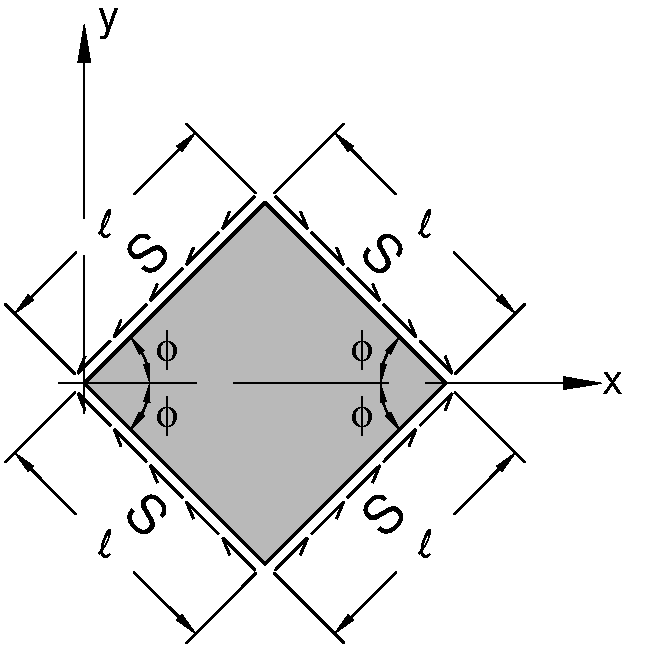
\includegraphics[width=7cm]{wedge.pdf}
\caption{2D Self-equilibrated wedge.}
\label{fig:WEDGE}
\end{figure}

Under plane strain conditions the general 3D stress equilibrium equations (see \cref{eq:pde}) reduce to:
\begin{equation}
\begin{aligned}
&\pdv{\sigma_{xx}}{x}+\pdv{\tau_{xy}}{y}=0\\
&\pdv{\tau_{xy}}{x}+\pdv{\sigma_{yy}}{y}=0
\end{aligned}
\label{eq:equilibrium}
\end{equation}

while the kinematic relation (\cref{eq:kin}) reads

\begin{equation}
\begin{aligned}
\epsilon_{xx}&=\pdv{u}{x}\\
\epsilon_{yy}&=\pdv{v}{y}\\
\gamma_{xy}&=\pdv{u}{y} + \pdv{v}{x}
\end{aligned}
\label{eq:strain}
\end{equation}
where $u$ and $v$ are the horizontal and vertical displacements respectively.

\subsubsection*{Stress field}

The stress field can be obtained by simple inspection from the traction boundary conditions prescribed over the inclined surfaces yielding;

\begin{align*}
\sum F_x &= 0 \longrightarrow - \ell S\cos(\phi)  + \sigma_{xx}\ell \sin(\phi) = 0\\
\sum F_y &= 0 \longrightarrow - \ell S\sin(\phi) - \sigma_{yy}\ell \cos(\phi)=0
\end{align*}

and the following stress solution:

\begin{equation}
\begin{aligned}
\sigma_{xx}& = S \cot(\phi)\\
\sigma_{yy}& = -S\tan(\phi)\\
\tau_{xy}& = 0.
\end{aligned}
\label{eq:solution}
\end{equation}

In \cref{eq:solution} the condition $\tau_{xy}=0$ is due to the symmetries in the problem.

\subsubsection*{Traction boundary conditions}
Let us verify that the above stress solution satisfies the traction BC using the expression:

\[t_i^{\hat n} = \sigma _{ij} \hat n_{ij}.\]

Denoting the outward normals to the inclined surfaces of the wedge by $\hat{n}^1$,  $\hat{n}^2$, $\hat{n}^3$, $\hat{n}^4$ these are given by;
\begin{align*}
\hat{n}^1 &= -\sin(\phi)\hat{e}_{x}+\cos(\phi)\hat{e}_{y}\\
\hat{n}^2 &= -\sin(\phi)\hat{e}_{x}-\cos(\phi)\hat{e}_{y}\\
\hat{n}^3 &= +\sin(\phi)\hat{e}_{x}+\cos(\phi)\hat{e}_{y}\\
\hat{n}^4 &= +\sin(\phi)\hat{e}_{x}-\cos(\phi)\hat{e}_{y} \enspace
\end{align*}

where $\hat{e}_{x}$ and $\hat{e}_{y}$ are the reference unit vectors. Now, the components of the traction vector follow directly like

\[t_{i} = \sigma_{ij}\hat{n}_{j}\]

then over the face with normal $\hat{n}^1$ we have
\begin{align*}
t_{x} &= -S\cos(\phi)\\
t_{y} &= -S\sin(\phi)
\end{align*}
similarly, over the face with normal $\hat{n}^2$
\begin{align*}
t_{x} &= -S\cos(\phi)\\
t_{y} &= +S\sin(\phi)
\end{align*}
over the face with normal $\hat{n}^3$ 
\begin{align*}
t_{x} &= +S\cos(\phi)\\
t_{y} &= -S\sin(\phi)
\end{align*}
and finally, over the face with normal $\hat{n}^4$;
\begin{align*}
t_{x} &= +S\cos(\phi)\\
t_{y} &= +S\sin(\phi) \enspace .
\end{align*}

\subsubsection*{Strain field}
The strain field can be obtained after using the stress solution found in \cref{eq:solution} together with the constitutive law given by \cref{eq:Hooke} which for a plane strain idealization takes the form:

\begin{equation}
\begin{aligned}
\epsilon_{xx}& = \frac{1}{E}(\sigma_{xx} - \nu \sigma_{yy}) \\
\epsilon_{yy}& = \frac{1}{E}(\sigma_{yy} - \nu \sigma_{xx}) \\
\gamma_{xy}& = \frac{\tau _{xy}}{\mu}
\end{aligned}
\label{eq:cons model}
\end{equation}

which for the particular case yields;


\begin{equation}
\begin{aligned}
\epsilon_{xx}& = +\dfrac{S}{E}\left[\cot(\phi)+\nu \tan(\phi)\right] = +\dfrac{S}{E}K_{1}(\nu , \phi)\\
\epsilon_{yy}& = -\dfrac{S}{E}\left[\tan(\phi)+\nu \cot(\phi)\right] = -\dfrac{S}{E}K_{2}(\nu , \phi)\\
\gamma_{xy}& = 0.
\end{aligned}
\label{eq:strain part}
\end{equation}

\subsubsection*{Displacement field}
The displacement field is obtained after direct integration of the strains after using the fact that:

\[du_i=\epsilon_{ij}dx_j + \omega_{ij}dx_j\]

and the condition $\omega_{xy}=0$ also due to symmetries , as follows:

\begin{align*}
u &= +\dfrac{S}{E} K_{1}(\nu , \phi)x + A\\
v &= -\dfrac{S}{E} K_{2}(\nu , \phi)y + B
\end{align*}

and where $A$ and $B$ are integration constants.

From the condition $u=0$ at $x=\ell\cos(\phi)$ we have that $A=-\dfrac{S}{E} K_{1}(\nu , \phi)\ell\cos(\phi)$ then it follows that
\[u=\dfrac{S}{E} K_{1}(\nu , \phi)(x-\ell\cos(\phi)).\]

Similarly, from the condition $v=0$ at $y=0$ we have that $B=0$ from which
\[v=-\dfrac{S}{E} K_{2}(\nu , \phi)y\]

%%
\subsection{Variational formulation}
In this section we formulate the boundary value problem using the approach of the calculus of variations in which the governing PDEs and boundary conditions are obtained after finding the minimum (or maximum) of a functional according to a variational principle\footnote{According to Wikipedia \cite{wiki:variational_principle}

\begin{quotation}
A variational principle is a scientific principle used within the calculus of variations, which develops general methods for finding functions which minimize or maximize the value of quantities that depend upon those functions. For example, to answer this question: ``What is the shape of a chain suspended at both ends?" we can use the variational principle that the shape must minimize the gravitational potential energy.

According to Cornelius Lanczos, any physical law which can be expressed as a variational principle describes an expression which is self-adjoint. These expressions are also called Hermitian. Such an expression describes an invariant under a Hermitian transformation.
\end{quotation}}.
%%
We will see that the weak form (and therefore also the strong form) can be obtained alternatively through the process of finding extreme values for a functional. We will illustrate this idea for the general case of theory of elasticity and then we will present particular examples.

\subsubsection*{Some vague definitions in the calculus of variations}
In variational calculus a {\bf functional} can be understood as a ``function" having as independent variables or arguments a space of vector functions and producing as a result (or dependent variable) a scalar. For instance, in the particular case of the theory of elasticity such a ``function" corresponds to the total potential energy functional $\Pi$ given by;
\begin{equation}\label{eq:Potential}
    \Pi(u_i) = \frac{1}{2}\int\limits_V \sigma_{ij}\varepsilon_{ij}\dd{V}  - \int\limits_V f_i\, u_i\dd{V}  - \int\limits_S t_i^{(n)} u_i\dd{S}
\end{equation}
and where the first term in the left hand side corresponds to the internal strain energy, while the last two terms are the work done by the external body and traction forces. The above functional has as independent variables the displacement vector and its spatial derivatives. This is indicated by the presence of the displacement vector $u_i$ in the expression $\Pi(u_i)$.

In variational calculus we are interested in finding a function $u_i$ that renders the functional $\Pi$ a maximum or a minimum. In loose terms, the analogous to the differential operator in calculus of functions is now termed the variational operator $\var$ (i.e., $\var$ is analogous to $\pdv{x_i}$). As such $\var{\Pi}$ acts over the function $u_i$ and its derivatives as follows
\[\var{\Pi}  = \pdv{\Pi}{u_i}\var{u_i} + \pdv{\Pi}{\left( \pdv{u_i}{x_j}\right)} \delta\left(\pdv{u_i}{x_j}\right) + \cdots + \pdv{\Pi}{\left( \pdv{^{n}u_i}{x_j \cdots \partial x_k}\right)} \delta\left( \pdv{^{n}u_i}{x_j \cdots \partial x_k}\right) \enspace .\]

The following rules apply to the variational operator $\delta$:
\begin{itemize}
\item For functionals $\Pi$ and $\Phi$ it follows that \[\var(\Pi  + \Phi) = \var{\Pi}  + \var{\Phi}\]
\item For functionals $\Pi$ and $\Phi$ it follows that \[\var(\Pi \Phi ) = \var{\Pi} \Phi  + \Pi \var{\Phi}\]
\item For a functional $\Pi$ and an integer $n$ it follows that \[\var(\Pi^n) = n(\Pi^{n - 1})\var{\Pi}\]
\item For a functional $\Pi$ it follows that \[\var{\int \Pi \dd{x}}  = \int \var{\Pi} \dd{x} \]
\end{itemize}

If the variational operator is applied to the functional $\Pi(u_i)$ it produces functions or variations in $u_i$ which are arbitrary and such $\var{u_i} \in V$ and $\var{u_i} = 0$ in $S_u$.

To find an extreme function in the calculus of variations we proceed like in differential calculus. Here we compute the first variation of the functional $\var{\Pi}$ and solve the variational equation
\begin{equation}\label{eq:vareq}
    \delta \Pi  = 0
\end{equation}
in the unknown function $u_i$. 

In the particular case of the total potential energy functional $\Pi$ this yields
\begin{equation}\label{eq:ClaPVW}
    \int\limits_V \sigma _{ij}\var{\varepsilon_{ij}}\dd{V}  - \int\limits_V f_i var{u_i} \dd{V}  - \int\limits_{S_t} t_i^{(n)} \var{u_i}\dd{S}  = 0
\end{equation}
where we recognize the weak form of the BVP stated previously. It becomes evident that the functions $\delta {u_i}$ in \cref{eq:ClaPVW} play the role of the test functions $w_i$ introduced in the weak form. On the other hand, since we have already shown that the weak and strong forms are equivalent we conclude that having the functional and the essential boundary conditions is equivalent to having the strong form of the problem.


\subsubsection*{Principle of minimum potential energy}
In the theory of elasticity the total potential energy $\Pi$ is the result of adding the elastic strain energy which is stored in the body upon deformation and the potential energy (work) imparted to the body by the applied forces. The principle states that the body is in equilibrium when this total potential energy reaches a minimum. This is equivalent to stating that an equilibrium configuration is attained when an infinitesimal variation from the position of minimum potential energy involves null changes in energy. This implies the variational condition:
\begin{equation}\label{vareq2}
    \delta \Pi  = 0.
\end{equation}

The above principle leads to the so-called principle of virtual displacements stated as follows\footnote{see Bathe pp 156}:
``The equilibrium of the body requires that for any compatible small virtual displacements satisfying the condition of being zero at $S_u$, imposed on the body in its state of equilibrium, the total internal virtual work is equal to the total external virtual work"
\[\int\limits_V \sigma _{ij}\var{\varepsilon_{ij}}\dd{V}  - \int\limits_V f_i\delta u_i\dd{V}  - \int\limits_{S_t} t_i^{(n)}\var{u_i}\dd{S}  = 0\]
where $\var{u_i}$ are the virtual displacements and $\var{ \varepsilon_{ij}}$ are the corresponding virtual strains.

Comparing the virtual work principle with the weak formulation given in \cref{eq:weak} we identify $\var{u_i}$ with the test functions $w_i$. As such the PVW takes the form of a powerful tool to test if a body is in equilibrium for a given solution (represented by the trial functions). In what follows we illustrate the use of the principle through some examples corresponding to problems in Bathe's textbook.

\subsubsection*{Problem 3.15 from Finite Element Procedures}
Establish the differential equation of equilibrium of the problem shown and the boundary conditions. Determine whether the differential operator of the problem is symmetric and positive definite and prove your answer.\cite{book:bathe}

\begin{figure}[H]
    \centering
    \includegraphics[width=10cm]{{Bathe3.15}.pdf}
    \caption{Rod with varying cross-sectional area. The Young's modulus is E.}
    \label{fig:bathe3.15}
\end{figure}


\begin{align*}
\Pi &= \frac{1}{2}\int\limits_0^L \sigma_{xx}\varepsilon_{xx}A(x)\dd{x} + \frac{1}{2}ku_0^2 - R u_L \\
 &= \frac{1}{2}\int\limits_0^L EA(x)\left( \dv{u}{x}\right)^2 \dd{x} + \frac{1}{2}ku_0^2  - R u_L \enspace.
\end{align*}

The first variation for this functional is
\[\var{\Pi}  = \int\limits_0^L EA(x)\dv{u}{x}\dv{\var{u}}{x}\dd{x} + k u_0\var{u_0}  - R\var{u_L} \enspace .\]

If we integrate by parts, we obtain
\[\var{\Pi}  =  - \int\limits_0^L \dv{x}\left[EA(x)\dv{u}{x}\right]\var{u}\dd{x} + \left. EA(x)\dv{u}{x}\var{u} \right|_0^L + k{u_0}\var{u_0}  - R\var{u_L}\]
from which
\begin{align*}
&\dv{x}\left[EA(x)\dv{u}{x}\right] = 0\\
&\left. EA(x)\dv{u}{x}\right|_{x=0} = k u_0\\
&\left. EA(x)\dv{u}{x}\right|_{x=L} = R
\end{align*}


\subsubsection*{Problem 4.35-The Hu-Washizu Variational Principle}
Consider the Hu-Washizu functional:
\begin{equation}
\Pi^* = \Pi  - \intL_V \lambda_{ij}^\varepsilon (\varepsilon_{ij} - L_{ijk} u_k)\dd{V}  - \intL_{S_u} \lambda_i^u(u_i^{S_u} - \bar{ u}_i)\dd{S}
\label{eq:Hu}
\end{equation}

where
\begin{itemize}
\item $\Pi$: is the potential energy functional.
\item $L_{ijk}$ is a differential operator such $\varepsilon_{ij} = L_{ijk} u_k$.
\item $S_u$ surface where essential boundary conditions are prescribed.
\item $\lambda_{ij}^\varepsilon $ and $\lambda_i^u$ are Lagrange multipliers.
\end{itemize}

Using the condition $\var{\Pi} = 0$ derive for the interior of the body the equilibrium equations
\[\sigma_{ij,j} + f_i = 0\]
the strain-displacement relationship
\[\varepsilon_{ij} = L_{ijk} u_k\]
and the constitutive equation
\[\sigma_{ij} = C_{ijkl} \varepsilon_{kl}\]
and at the surface of the body the relation between the stress tensor and the applied tractions vector at $S_t$
\[t_i = \sigma_{ij} n_j\]
the relation between the stress tensor and the unknown tractions vector (or reactions) at $S_u$
\[t_i = \tilde{\sigma_{ij}} n_j\]
and the essential boundary condition at $S_u$
\[u_i = \tilde{u}_i\]
We want to determine the so-called Euler equations resulting from the condition $\var{\Pi}^* = 0$. Applying the variational operator we have:
\begin{equation}
\begin{aligned}
\var{\Pi}^*& = \var{\Pi}  - \intL_V \var{\lambda}_{ij}^{\varepsilon}  (\varepsilon_{ij} - L_{ijk} u_k)\dd{V}- \intL_V \lambda_{ij}^\varepsilon (\var{\varepsilon}_{ij} - L_{ijk}\var{u}_k)\dd{V} \\
&-\intL_V \var{\lambda}_i^u (u_i^{S_u} - \bar u_i)\dd{S} - \intL_V \lambda _i^u \var{u}_i^{S_u} \dd{S}
\end{aligned}
\end{equation}
and
\begin{equation}
\begin{aligned}
\var{\Pi}^* &= \intL_V C_{ijkl} \varepsilon_{kl} \var{ \varepsilon}_{ij}\dd{V} - \intL_{S_t} t_i \var{u_i} \dd{S}  - \intL_V f_i \var{u_i}\dd{V} - \intL_V \lambda_{ij}^{\varepsilon} \var{\varepsilon}_{ij}\dd{V}  + \intL_V \lambda_{ij}^{\varepsilon} L_{ijk}\var{u_k}\dd{V}\\
&- \intL_V \delta \lambda_{ij}^\varepsilon (\varepsilon_{ij} - L_{ijk} u_k)\dd{V} - \intL_S \var{\lambda}_i^u (u_i^{S_u} - \bar {u}_i)\dd{S} - \intL_{S_u} \lambda _i^u\var{u_i}\dd{S} = 0
\end{aligned}
\end{equation}
using
\[\intL_V (\lambda_{ij}^\varepsilon \var{u_i}){,_j}\dd{V} =  \intL_V \lambda_{ij}^\varepsilon \var{u}_{i,j}\dd{V}  + \intL_V \lambda_{ij,j}^\varepsilon \var{u_i}\dd{V} \]

In the above we can write
\begin{align*}
\intL_V \lambda_{ij}^\varepsilon L_{ijk}\var{u_k}\dd{V} & = \intL_V (\lambda_{ij}^\varepsilon \var{u_i})_{,j}\dd{V} - \intL_V \lambda_{ij,j}^\varepsilon \delta {u_i}\dd{V}\\
& = \intL_{S_t} \lambda_{ij}^\varepsilon \var{u_i}\hat {n}_j\dd{S}  - \intL_V \lambda_{ij,j}^\varepsilon \var{u_i}\dd{V}
\end{align*}
therefore
\begin{align*}
\delta \Pi^* &= \intL_V (C_{ijkl}\varepsilon_{kl} - \lambda_{ij}^\varepsilon) \var{\varepsilon}_{ij}\dd{V} - \intL_{S_t} t_i \var{u}_i\dd{S} - \intL_V f_i \var{u}_i\dd{V} + \intL_{S_t} \lambda_{ij}^\varepsilon \var{u_i}\hat{n}_j\dd{S}  - \intL_V \lambda_{ij,j}^\varepsilon \delta {u_i}\dd{V}\\
&- \intL_V \delta \lambda _{ij}^\varepsilon (\varepsilon_{ij} - L_{ijk} u_k)\dd{V}  - \intL_{S_u} \var{\lambda}_i^u (u_i^{S_u} - \bar{u}_i)\dd{S} - \intL_{S_u} \lambda_i^u \var{u_i} \dd{S}  = 0\\
&= \intL_V (C_{ijkl}\varepsilon_{kl} - \lambda_{ij}^\varepsilon) \var{\varepsilon}_{ij}\dd{V}
+ \intL_{S_t} (\lambda_{ij}^\varepsilon \hat{n}_j - t_i)\delta {u_i}\dd{S}\\
&- \intL_V (\lambda_{ij,j}^\varepsilon  + f_i) \var{u_i}\dd{V}
- \intL_V (\varepsilon_{ij} - L_{ijk} u_k) \var{\lambda} _{ij}^\varepsilon\dd{V}
- \intL_{S_u} (u_i^{S_u} - \bar{u}_i) \var{\lambda}_i^u\dd{S}  - \cancel{\intL_{S_u} \lambda _i^u \var{u}_i^{S_u}\dd{S}} = 0
\end{align*}

Now, imposing the conditions $\var{\varepsilon}_{ij} \neq 0$, $\var{\lambda}_{ij}^\varepsilon  \neq 0$, $var{u}_i \neq 0$ in $S_t$, $\var{u}_i \neq 0$ in $V$ and $\var{\lambda}_i^u \neq 0$ in $S_u$ we have
\begin{align}
&\lambda_{ij}^\varepsilon  = C_{ijkl} \varepsilon_{kl}\\
&\varepsilon_{ij} = L_{ijk} u_k\\
t_i &= \lambda_{ij}^\varepsilon \hat{n}_j\\
&\lambda_{ij,j}^\varepsilon  + {f_i} = 0\\
&u_i^{S_u} = \bar{u}_i \enspace .
\end{align}

\subsection{Weighted residual methods}
This section introduces the concept of residual or difference from zero in a differential equation once its solution is aproximated numerically. For that purpose we will take as prototype equation the one obtained as our general model of BVP (see \cref{eq:GenPDE}) and recalled here for completeness:

\begin{equation}
\rho(\vb x) \pdv{u(\vb x, t)}{t} + \mathcal{L}u(\vb x, t) = \rho (\vb x)F(\vb x, t) \enspace .
\label{eq:GenPDE2}
\end{equation}


We will assume that the actual solution to the generalized BVP given by \cref{eq:GenPDE2} is approximated by the numerically derived solution $\tilde u(\vb{x})$ through a superposition like

\begin{equation}
\tilde u (\vb{x}) = {N^I}(\vb{x}){u^I}
\label{basicsuper}
\end{equation}

where ${N^I}(\vb{x})$ are interpolating functions and $I$ denotes a superposition index  varying like $I=1,2,...,K$ with $K$ being the number of points where the solution is known. In what follows we will use $u(\vb{x})$ instead of $\tilde u (\vb{x})$ but will keep in mind that we are actually using the approximation given by \cref{basicsuper}. Similarly, in order to keep the discussion simple for the time being we will drop the time effects reducing the generailzed P.D.E to the simple form:

\begin{equation}
\mathcal{L}u(\vb x, t) = \rho (\vb x)F(\vb x, t) \enspace .
\label{eq:GenPDE3}
\end{equation}



Now, since we are using the approximation given by \cref{basicsuper} this equation is not strictly satisifed but instead we will have the following "unbalanced" condition

\[Lu(\vb{x},t) - \rho (\vb{x})F(\vb{x}, t) \equiv R \ne 0\]

where the term $R$ corresponds to a residual error which is to be distributed throughout the solution domain. The so-called weighted residual methods differ in the form in which they distribute the residual between the different $K$ points conforming the computational domain.

Using \cref{basicsuper} in \cref{eq:GenPDE2} and the linearity in the differential operator yields;

\[R = \mathcal{L}({N^P}){u^P} - \rho F.\]

In what follows we will consider different strategies to distribute or weight the residual $R$ over the computational domain.

\subsubsection{Galerkin}
In the Galerkin scheme the interpolation functions are used also as weighting functions leading to:

\[\int\limits_V {{N^Q}RdV = 0} \]

or explicitly;

\begin{equation}
\int\limits_V {{N^Q} \mathcal{L} ({N^P})dV} {u^P} = \int\limits_V {{N^Q}\rho FdV}
\label{Galer}
\end{equation}



Imposing \cref{Galer} in the $K$ points conforming the computational domain or equivalently ranging $Q$ from $1$ to $K$ leads to the following system of algebraic equations;

\begin{equation}
{K^{QP}}{U^P} = {f^Q}
\label{DGaler}
\end{equation}

where $U^P$ is a vector that stores the point values of the function $u$ along te $K$ points of the computational domain, while $f^Q$ stores the corresponding point excitations.

\subsubsection{Least squares method}
In this method the integral of the square of the residual is minimized with respect to the $K$ point parameters or nodal values of the function. Accordingly;

\[\frac{\partial }{{\partial {u^I}}}\int\limits_V {{R^2}dV}  = 0\]

\[\frac{\partial }{{\partial {u^I}}}\int\limits_V {{{[\mathcal{L}({N^P}{u^P}) - \rho F]}^2}dV}  = 0\]

\[\int\limits_V {[\mathcal{L}({N^P}{u^P}) - \rho F]L({N^I})dV}  = 0\]

\[\int\limits_V {L({N^I})L({N^P})dV} {u^P} - \rho \int\limits_V {L({N^I})FdV = 0} \]

which can be written like;

\begin{equation}
{K^{IP}}{U^P} = {f^I}
\label{Dsquares}
\end{equation}

\subsubsection{Collocation method}
Zero values of the residual are directly imposed over the $K$ points of the computational domain;

\[\mathcal{L}({N^I}){u^I} - \rho F = 0\]

\[L[{N^I}({x^J})]{u^I} - \rho F({x^J}) = 0\]

where $J$ ranges between $1$ and $K$ leading to the system;

\begin{equation}
{K^{IP}}{U^P} = {f^I}
\label{DColo}
\end{equation}

\subsubsection{Subdomian method}
The zero value of the residual is imposed upon $K$ subdomains.

\[\int\limits_{{V^I}} {\mathcal{L}({N^P})d{V^I}{u^P}}  - \rho \int\limits_{{V^I}} {Fd{V^I}}  = 0 \quad \quad I=1,...,K.\] For instance, for the $N$-th element it follows that ;

\[\int\limits_{{V^N}} {\mathcal{L}({N^P})d{V^N}{u^P}}  - \rho \int\limits_{{V^N}} {Fd{V^N}}  = 0 \quad \quad P=1,...,K.\]

Applying the equation over the $K$ subdomains leads to the discrete system;


\begin{equation}
{K^{IP}}{U^P} = {f^I} \quad \quad I=1,...,K.
\label{DColo}
\end{equation}

\subsubsection{Ritz method} It operates directly upon the variational statement of the problem. For a given functional;

\[\Pi  = \Pi ({N^Q}{u^Q})\]

the variational equation reads;

\[\delta \Pi  \equiv \frac{{\partial \Pi }}{{\partial {u^Q}}}\delta {u^Q} = 0\]

from which

\[\frac{{\partial \Pi }}{{\partial {u^Q}}} = 0.\]

\subsubsection*{Generalized parabolic equation.}
Let us consider the case of the generalized parabolic equation and its discretization following the Galerkin method;

\[\rho(\vb x) \pdv{u(\vb x,t)}{t} + \mathcal{L}u(\vb x, t) = 0\]

which can also be written using indicial notation;

\[\frac{\partial }{{\partial {x_i}}}\left[ {p(x)\frac{{\partial u}}{{\partial {x_i}}}} \right] + q(x)u + \rho \frac{{\partial u}}{{\partial t}} = \rho F.\]

Assuming for simplicity that $p(x)=1$ yields;

\[ - \int\limits_V {{N^P}N_{,ii}^Q} dV{u^Q} + \int\limits_V {q{N^P}{N^Q}dV{u^Q}}  + \rho \int\limits_V {{N^P}{N^Q}dV{v^Q}}  - \rho \int\limits_V {{N^P}FdV = 0} \]

\[\int\limits_V {N_{,i}^PN_{,i}^Q} dV{u^Q} - \int\limits_S {{N^P}N_{,i}^Q{{\hat n}_i}} dS{u^Q} + \int\limits_V {q{N^P}{N^Q}dV{u^Q}}  + \rho \int\limits_V {{N^P}{N^Q}dV{v^Q}}  - \rho \int\limits_V {{N^P}FdV = 0} \]

\[\int\limits_V {\left( {N_{,i}^PN_{,i}^Q + q{N^P}{N^Q}} \right)dV{u^Q}}  + \rho \int\limits_V {{N^P}{N^Q}dV{V^Q}}  = \int\limits_S {{N^P}N_{,i}^Q{{\hat n}_i}} dS{u^Q} + \rho \int\limits_V {{N^P}FdV} \]

which can be written in discrete form;

\[{K^{PQ}}{U^Q} + {C^{PQ}}{V^Q} = {f^p}\]



\subsubsection*{Navier equations.}
In this case the differential equations are written as
\[(\lambda  + \mu ){u_{j,ij}} + \mu {u_{i,jj}} + {f_i} = 0 \enspace .\]

We can write the differential operator as
\[L_{ij} \equiv (\lambda  + \mu )\pdv[2]{}{x_i}{x_j} + \mu \pdv[2]{}{x_k}{x_k}\delta_{ij}\]

\begin{align*}
&r_i =  - f_i\\
&u_i = N_i^Q u^Q\\
&\mathcal{L}_{ij}(u_j) \equiv (\lambda  + \mu )(N_j^Q{u^Q})_{,ij} + \mu (N_j^Q{u^Q})_{,kk}\delta_{ij}\\
&\mathcal{L}_{ij}(u_j) \equiv (\lambda  + \mu )N_{j,ij}^Q u^Q + \mu N_{i,kk}^Q u^Q\\
&\mathcal{L}_{ij}(u_j) \equiv \mathcal{L}_{ij}(N_j^Q) u^Q \enspace .
\end{align*}

In the Galerkin scheme we use the trial function as weighting function.
\[R_i \equiv L_{ij}(N_j^Q) u^Q + f_i\]
and we state \dots

\[\int\limits_V {N_i^P{R_i}dV = 0} \quad \quad P=1,2,...,N. \]

\[\int\limits_V {N_i^P{\mathcal{L}_{ij}}(N_j^K)dV{u^K}}  + \int\limits_V {N_i^P{f_i}dV = 0} \]

\[(\lambda  + \mu )\int\limits_V {N_i^PN_{j,ij}^KdV{u^K}}  + \mu \int\limits_V {N_i^PN_{i,kk}^KdV{u^K}}  + \int\limits_V {N_i^P{f_i}dV = 0} \]

integrating by parts;

\begin{align*}
- (\lambda  + \mu )\int\limits_V {N_{i,j}^PN_{j,i}^KdV{u^K} + (\lambda  + \mu )\int\limits_S {N_i^PN_{j,i}^K{{\hat n}_j}dS{u^K} - \mu \int\limits_V {N_{i,k}^PN_{i,k}^KdV{u^K}} } } \\
+ \mu \int\limits_S {N_i^PN_{i,k}^K{{\hat n}_k}dS{u^K}}  + \int\limits_V {N_i^P{f_i}dV = 0}
\end{align*}

which can be written like;


\[{K^{PQ}}{U^Q} = {F^P}\]

where

\[{K^{PQ}} = (\lambda  + \mu )\int\limits_V {N_{i,j}^PN_{j,i}^QdV}  + \mu \int\limits_V {N_{i,k}^PN_{i,k}^QdV} \]

\[{F^P} = \int\limits_S {N_i^Pt_i^{(\hat n)}dS + \int\limits_V {N_i^P{f_i}dV = 0} } \]

\subsubsection*{The acoustic wave equation.}

\[\vec \nabla  \cdot \left[ {\frac{1}{\rho }\vec \nabla p(\vb{x})} \right] - \frac{\partial }{{\partial t}}\left( {\frac{1}{\lambda }\frac{{\partial \rho }}{{\partial t}}} \right) - q(\vb{x}) = 0\]

where we recognize;

\[\mathcal{L}() \equiv \vec \nabla  \cdot \left( {\frac{1}{\rho }\vec \nabla } \right) - \frac{\partial }{{\partial t}}\left( {\frac{1}{\lambda }\frac{\partial }{{\partial t}}} \right)\]

Let

\[p(x) = {N^K}{p^K}\]

then

\[\mathcal{L}(p) \equiv \vec \nabla  \cdot \left( {\frac{1}{\rho }\vec \nabla {N^K}{p^K}} \right) - \frac{\partial }{{\partial t}}\left( {\frac{1}{\lambda }\frac{{\partial {N^K}{p^K}}}{{\partial t}}} \right)\]

or in indicial notation

\[\mathcal{L}(p) \equiv {\left( {\frac{1}{\rho }N_{,i}^K} \right)_{,i}}{p^K} - \frac{\partial }{{\partial t}}\left( {\frac{1}{\lambda }\frac{{\partial {N^K}}}{{\partial t}}} \right){p^K}\]

which is equivalent to having;

\[\mathcal{L}(p) \equiv \mathcal{L}({N^K}){p^K}\]

using the trial functions as weighting functios and recalling the definition of the residual which in this case reads;

\[R = \mathcal{L}({N^K}){p^K} - q\]

yields;

\[\int\limits_V {{N^J}RdV = 0} \quad \quad J=1,2,...,K \]

\[\int\limits_V {{N^J}L({N^K})dV{p^K}}  - \int\limits_V {{N^J}qdV}  = 0\]

\[\int\limits_V {{N^J}{{\left( {\frac{1}{\rho }N_{,i}^K} \right)}_{,i}}dV{p^K} - \int\limits_V {{N^J}\frac{\partial }{{\partial t}}\left( {\frac{1}{\lambda }\frac{{\partial {N^K}}}{{\partial t}}} \right)dV{p^K}} }  - \int\limits_V {{N^J}qdV}  = 0\]

Integrating by parts the first term on the R.H.S gives us;

\[ - \int\limits_V {N_{,i}^J\frac{1}{\rho }N_{,i}^KdV} {p^K} + \int\limits_S {{N^J}\frac{1}{\rho }N_{,i}^K{{\hat n}_i}dS{p^K}}  = \int\limits_V {{N^J}\frac{\partial }{{\partial t}}\left( {\frac{1}{\lambda }\frac{{\partial {N^K}}}{{\partial t}}} \right)dV{p^K}}  + \int\limits_V {{N^J}qdV} \]

\[\int\limits_V {N_{,i}^J\frac{1}{\rho }N_{,i}^KdV} {p^K} + \int\limits_V {{N^J}\frac{1}{\lambda }{N^K}dV{{\ddot p}^K}}  = \int\limits_S {{N^J}\frac{1}{\rho }N_{,i}^K{{\hat n}_i}dS{p^K}}  + \int\limits_V {{N^J}qdV} \]

\[{K^{JK}}{P^K} + {M^{JK}}{{\ddot P}^K} + {f^J} = 0\]


\section[Discretization of the PVW using FEM]{Discretization of the PVW via the FEM}

\subsection*{A simple spring-mass system}
The simple problem of a spring-mass system considered next resembles most of the algorithmic aspects of a finite element code with the advantage that the problem is already a discrete mechanical system. The problem consists of an assemblage of masses joined by different springs submitted to time varying loads. Each spring plays the role of a finite element and each mass is analogous to a nodal point in a finite element algorithm. For instance the full system may be like the one shown in \cref{fig:bathe}
\begin{figure}[H]
\centering
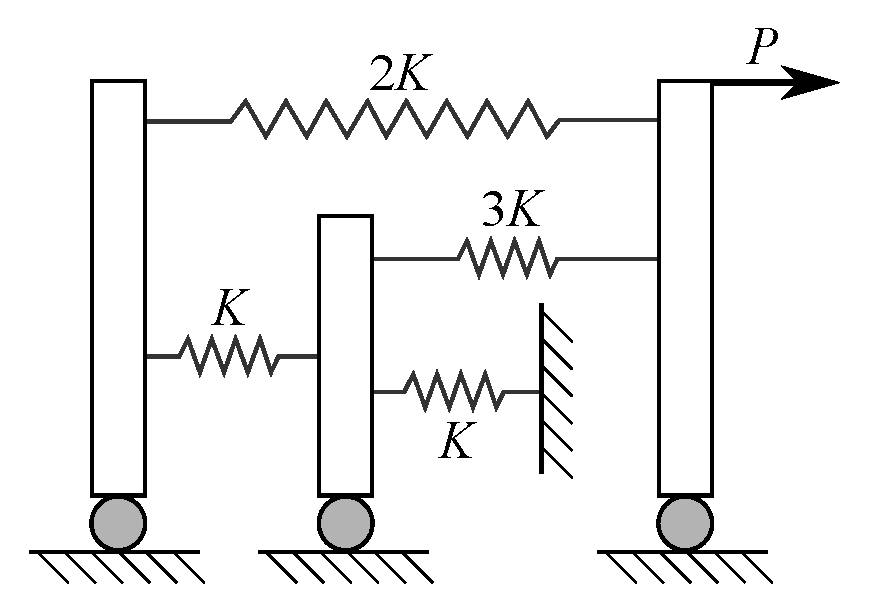
\includegraphics[width=10cm]{spring_system.pdf}
\caption{Typical assemblage of springs and masses.}
\label{fig:bathe}
\end{figure}


Consider a typical spring (finite element) like the one shown in \cref{fig:springel}
\begin{figure}[H]
\centering
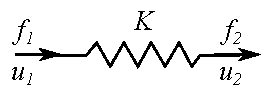
\includegraphics[width=8cm]{springel.pdf}
\caption{Typical spring element.}
\label{fig:springel}
\end{figure}

The relation between the force and the relative displacement can be written like
\[f_1 = K(u_1 - u_2)\]
and from equilibrium we have
\[f_1 + f_2 = 0\]
which yields the following force-displacement relationship for a typical spring element:
\begin{equation}
    \begin{Bmatrix}
        f_1\\
        f_2
    \end{Bmatrix} =
    K\begin{bmatrix}
          1.0 & -1.0\\
        - 1.0 & 1.0
    \end{bmatrix}
    \begin{Bmatrix}
        u_1\\
        u_2
    \end{Bmatrix}
    \label{eq:Kspring}
\end{equation}

On the other hand, the equilibrium equation for a typical mass with displacement $u_j$  (see \cref{fig:dclmass}) and attached to springs $i$ and $i+1$ reads
\begin{equation}
f_2^i + f_1^{i + 1} + m_j \dv{V_j}{t} = P_j.
\label{eq:equilmass}
\end{equation}
which can be written in terms of displacements using \cref{eq:Kspring} like
\[(K^i + K^{i + 1}) u_j - K^i u_{j - 1} - K^{i + 1} u_{j + 1} + m_j\dv{V_j}{t} = P_j .\]


\begin{figure}[H]
\centering
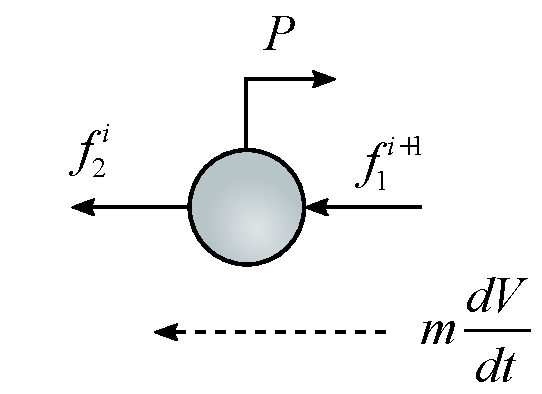
\includegraphics[width=8cm]{dcl_mass.pdf}
\caption{Free body diagram for a typical mass connected to springs $i$ and $i+1$.}
\label{fig:dclmass}
\end{figure}

Considering now the complete system of masses and springs leads to a system of linear equations of the form
\begin{equation}
\left[ {{K_G}} \right]\left\{ {{U_G}} \right\} + \left[ M \right]\left\{ {{A_G}} \right\} = \left\{ {{F_G}} \right\}.
\label{eq:global}
\end{equation}
where each equation represents the equilibrium of a given mass.

The system given by \cref{eq:global} can be solved in the displacements $U_G$. The pseudo-code shown in \cref{algo:springs} presents all the steps required to solve the problem in the context of the finite element method. In that code the so-called DME operator is an equation assembly array indicating how each element contributes to the global stiffness and mass matrix.

\begin{algorithm}[H]\label{algo:springs}
    \SetAlgoLined
    \KwData{Problem parameters; NUMNP, NUMEL, NMATP}
    \KwResult{Displacements and spring forces}
    Create $DM$E operator\;
    Assemble $K^G$, $F^G$\;
    \While{$j \leq 1, NUMEL$}{
        $K^G \leftarrow K^G+K^i$\\
        $F^G \leftarrow F^G+F^i$\\
    }
    Impose BCs\;
    Solve $[K^G]U=F^G$\\
    Find internal forces
    \caption{Springs Algorithm.}    
\end{algorithm}


\subsection{Basic elements of interpolation theory}
Let $f(x)$ be a function whose values are known at n discrete points ${x_1, x_2,...,x_n}$. We want to know (interpolate) the value of $f(x)$ at an arbitrary point $x \in \left[ {{x_1},{x_n}} \right]$.

\begin{figure}[h]
\centering
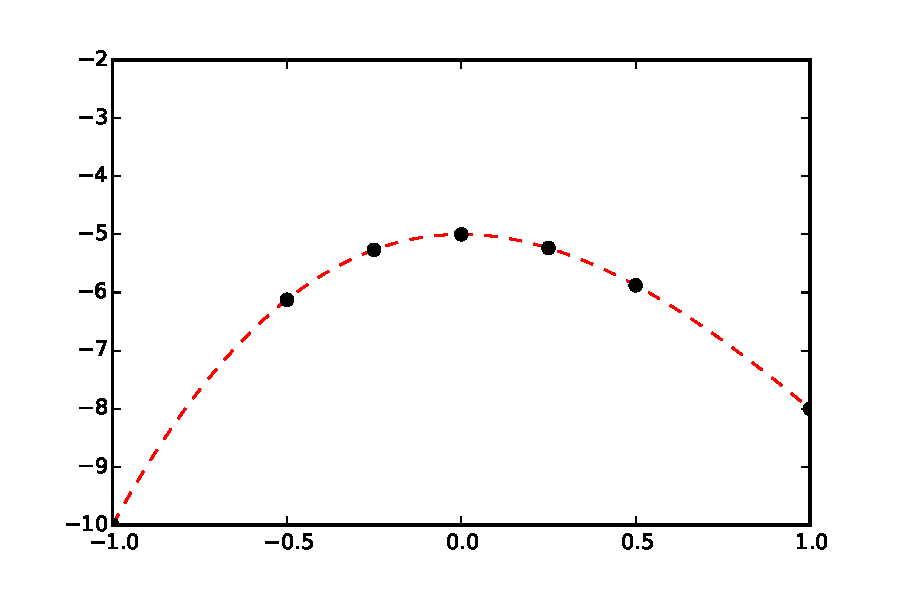
\includegraphics[width=12cm]{img/interpol1.pdf}
\caption{Global interpolation of a function}
\label{fig:interpol1}
\end{figure}

The process of interpolation or computation of the unknown value of $f(x)$ using the known values $\left\{ {{f^1},{f^2},...,{f^n}} \right\}$ involves two steps:

\begin{itemize}
\item[i]  Fitting an interpolating function to the known data points.
\item[ii] Evaluating the function at the arbitrary point.
\end{itemize}

We can (i) use all the n-data points and fit an $(n-1)$-th order polynomial (which is cumbersome and difficult to code) or (ii) split the domain in sub-intervals and use local polynomials within each sub-interval. This last approach involves only a couple of polynomials and it is easy to code, however it may have some continuity issues.

In finite element analysis local interpolation is used in order to proceed systematically. Local interpolation uses a finite number of nearest-neighbors and generates interpolated values $f(x)$ that do not in general have continuous first or higher derivatives.

\begin{figure}[h]
\centering
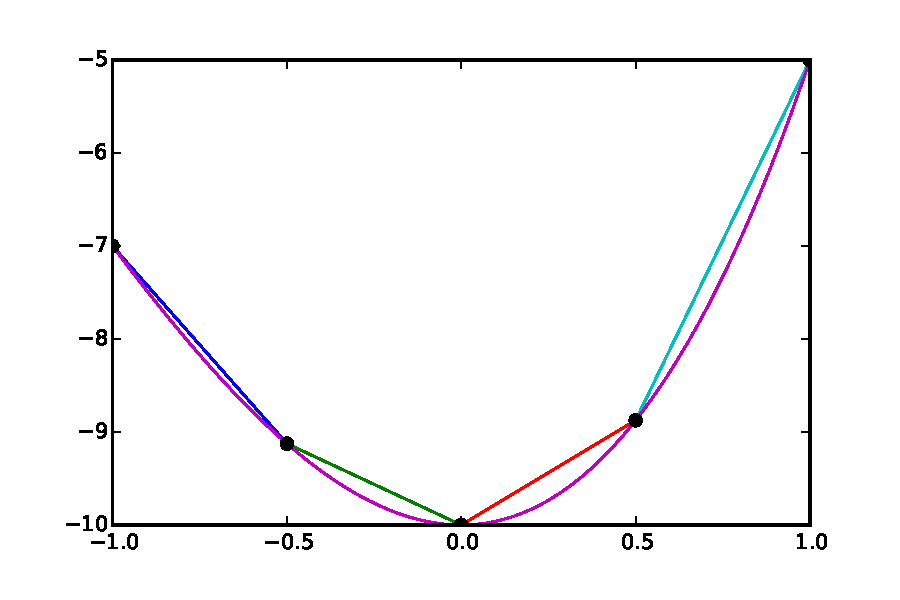
\includegraphics[width=12cm]{img/interpol2.pdf}
\caption{Local or piecewise interpolation of a function}
\label{fig:interpol2}
\end{figure}

\subsubsection{Lagrange interpolation theorem}
Given a set of n-points $\{ (x^1, y^1),\cdots,(x^n, y^n)\}$ where $y^n \equiv f({x^n})$ then: ``there exists a unique polynomial $p(x)$ of order at most $(n-1)$ such $p(x^I) = f(x^I)$ for $I=1,2,\cdots,n$". The polynomial is given by;
\begin{equation}\label{eq:pol}
  p(x^I) = L^I(x) f(x^I)  
\end{equation}
for $I=1,2,...,n$ where
\begin{equation}\label{eq:coef}
  L^I(x) = \prod_{\substack{J = 1\\ I \ne J}}^n \frac{(x - x^J)}{(x^I - x^J)}
\end{equation}
and where it should be noticed that
\[L^I(x^J) = \delta^{IJ}.\]

\subsubsection*{Example for n=3}
Consider the domain $[ - 1,1]$ and the data points at ${x^1} =  - 1.0$, ${x^2} =  + 1.0$ and ${x^3} = 0.0$. We have
\begin{align*}
& L^1(x) = \frac{(x - x^2)(x - x^3)}{(x^1 - x^2)(x^1-x^3)} \equiv  - \frac{1}{2}(1 - )x\\
& L^2(x) = \frac{(x - x^1)(x - x^3)}{(x^2 - x^1)(x^2 - x^3)} \equiv  + \frac{1}{2}(1 + x)x
\end{align*}
and
\[L^3(x) = \frac{(x - x^1)(x - x^2)}{(x^3 - x^1)(x^3 - x^2)} \equiv 1 - x^2.\]

The resulting interpolating polynomials $L^I(x)$ and the interpolating function  are shown in \cref{fig:pols} below
\begin{figure}[H]
  \centering
  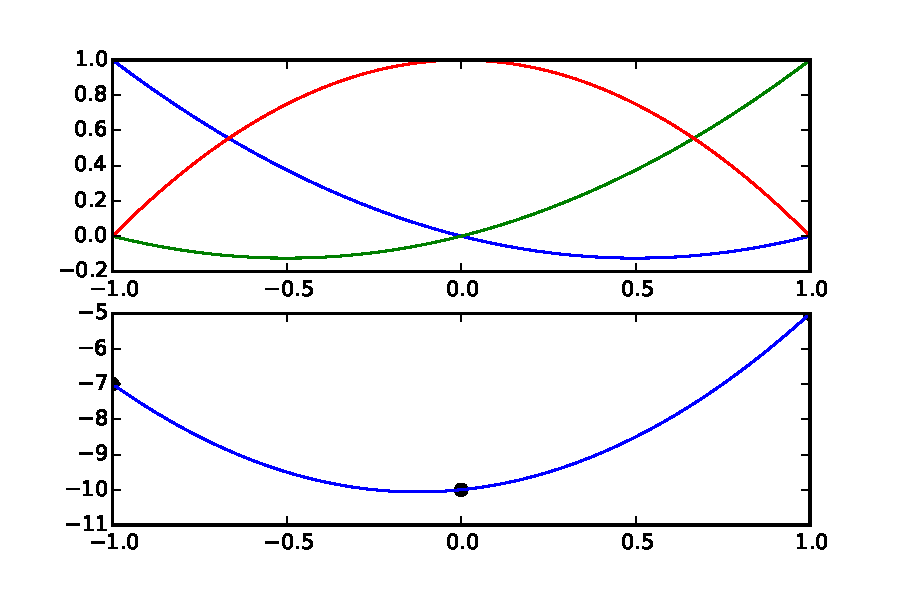
\includegraphics[width=16cm]{func.pdf}
  \caption{Interpolating polynomials and the resulting interpolating function}
  \label{fig:pols}
\end{figure}

\subsubsection*{Example: Interpolation of a function using a global and a local scheme}
Assume we have known values of the function:

\[f(x) = {x^3} + 4{x^2} - 10\]

in the interval $[-1.0, 1.0]$ and we wish to obtain an interpolated version of the function using different schemes.


\begin{figure}[H]
\centering
	\begin{subfigure}[b]{0.45\textwidth}\qquad
		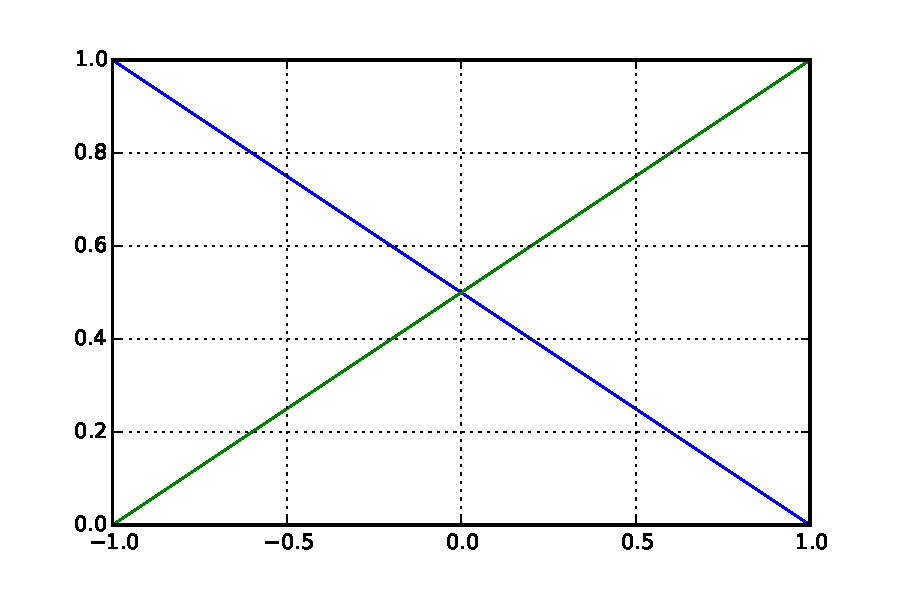
\includegraphics[width=\textwidth]{lineal.pdf}
		\caption{Interpolation polynomials. }
	\end{subfigure}\,
%
	\begin{subfigure}[b]{0.45\textwidth}\qquad
		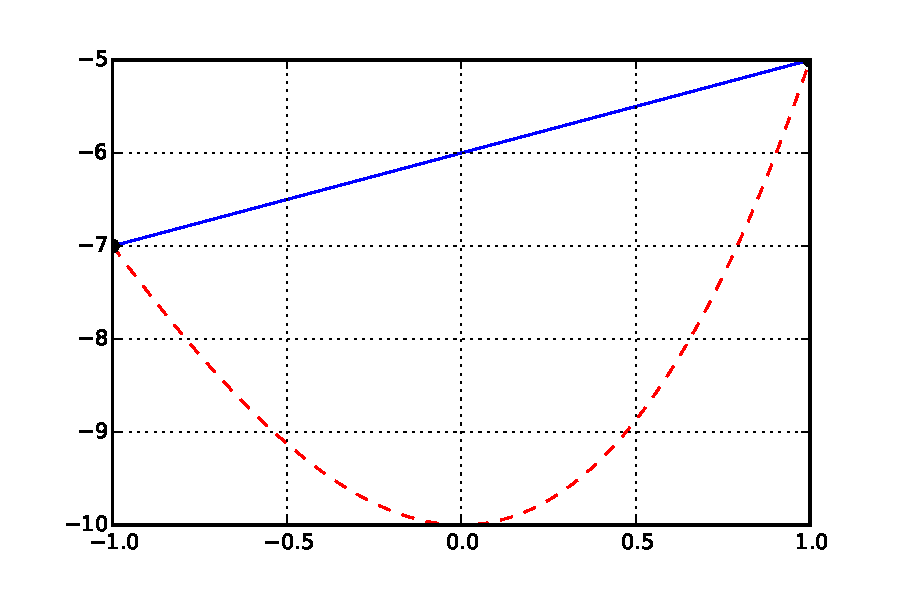
\includegraphics[width=\textwidth]{interlin.pdf}
		\caption{Actual and interpolated function.}
	\end{subfigure}\\
%
\centering
	\begin{subfigure}[b]{0.45\textwidth}\qquad
		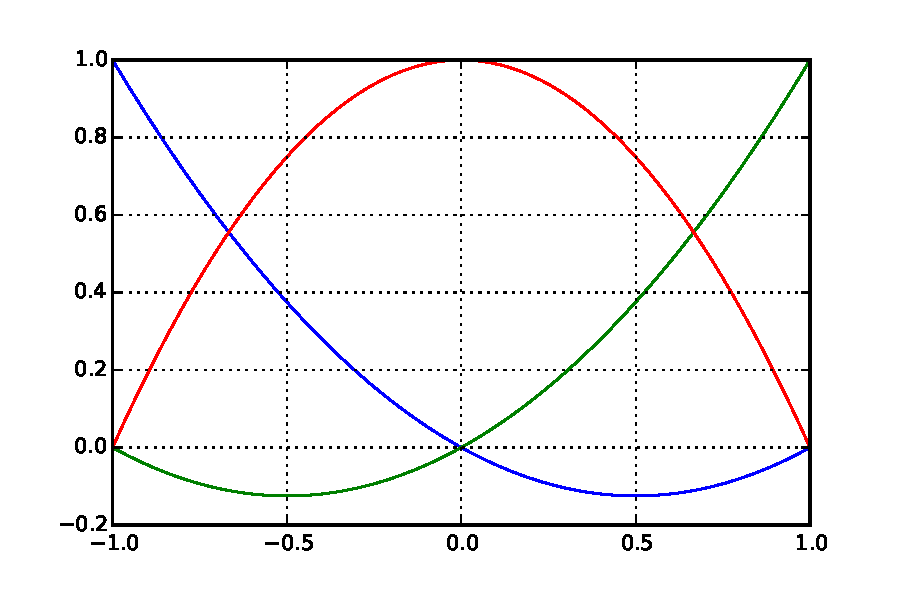
\includegraphics[width=\textwidth]{quadra.pdf}
		\caption{Interpolation polynomials.}
	\end{subfigure}\,
%
	\begin{subfigure}[b]{0.45\textwidth}\qquad
		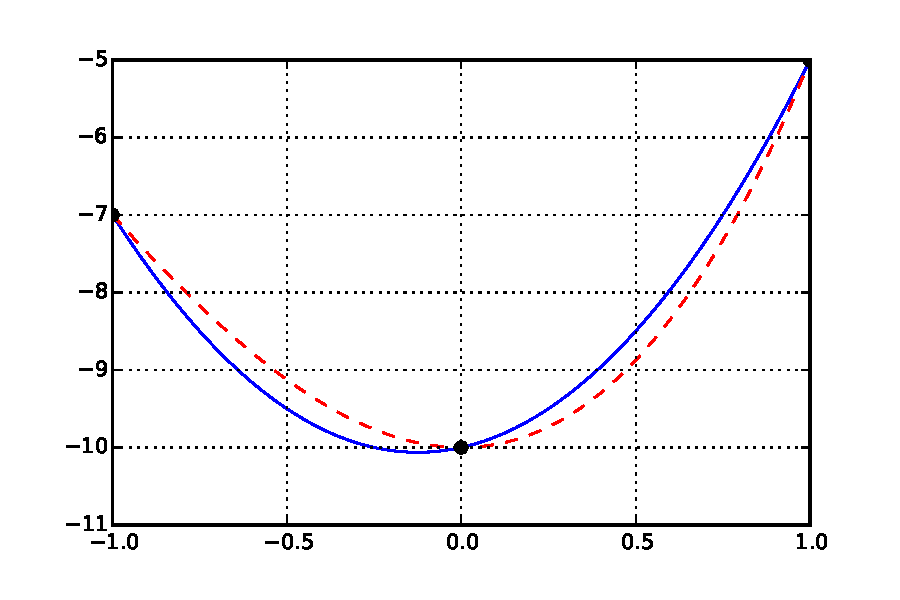
\includegraphics[width=\textwidth]{interqua.pdf}
		\caption{Actual and interpolated function.}
	\end{subfigure}\\
%
\centering
	\begin{subfigure}[b]{0.45\textwidth}\qquad
		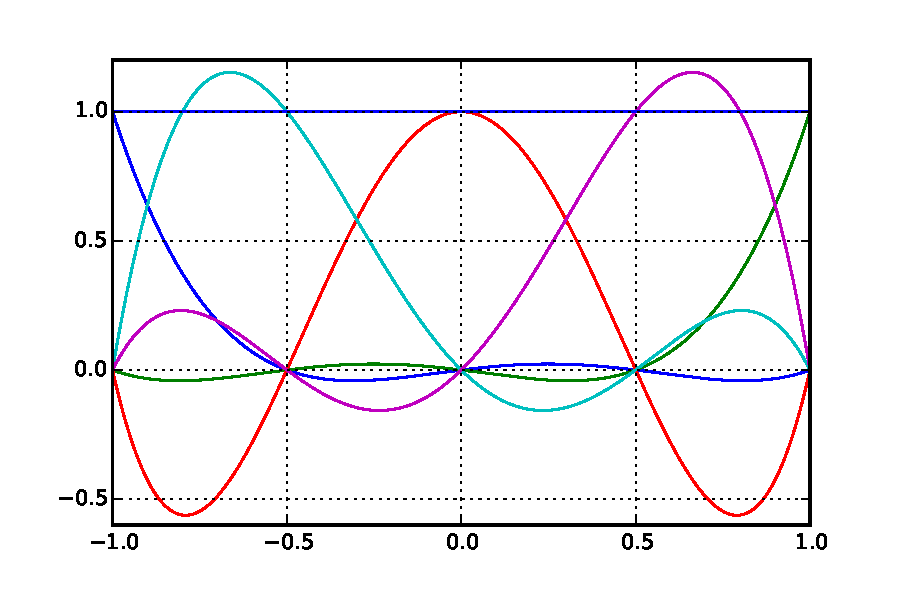
\includegraphics[width=\textwidth]{third.pdf}
		\caption{Interpolation polynomials.}
	\end{subfigure}\,
%
	\begin{subfigure}[b]{0.45\textwidth}\qquad
		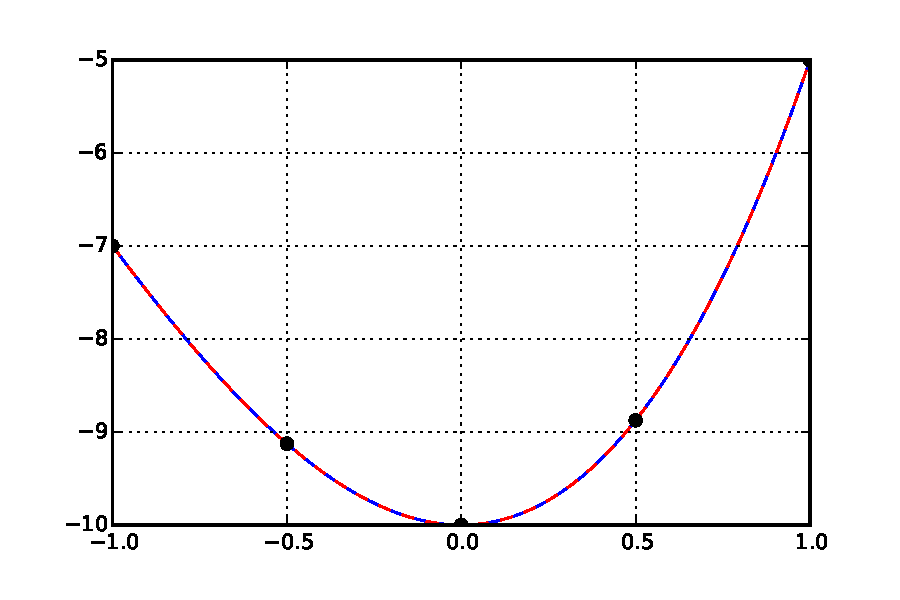
\includegraphics[width=\textwidth]{intertri.pdf}
		\caption{Actual and interpolated function.}
	\end{subfigure}
\caption{Lineal interpolation of the function $f(x) = {x^3} + 4{x^2} - 10$.}
\label{fig:several interpol}
\end{figure}

\Cref{fig:several interpol} shows the interpolating polynomials and the resulting function for the case of first, second and fourth order polynomials respectively. Similarly, the first order derivative obtained out of the interpolated function is displayed in \cref{fig:first der}. 

\begin{figure}[H]
\centering
	\begin{subfigure}[b]{0.45\textwidth}\qquad
		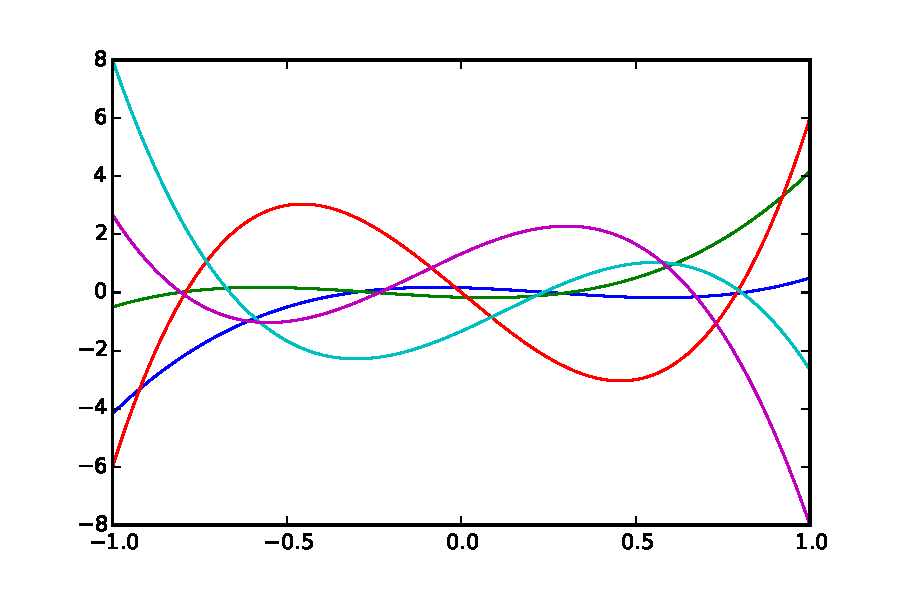
\includegraphics[width=\textwidth]{deriv2.pdf}
		\caption{First order derivatives of the interpolation polynomials. }
	\end{subfigure}\,
%
	\begin{subfigure}[b]{0.45\textwidth}\qquad
		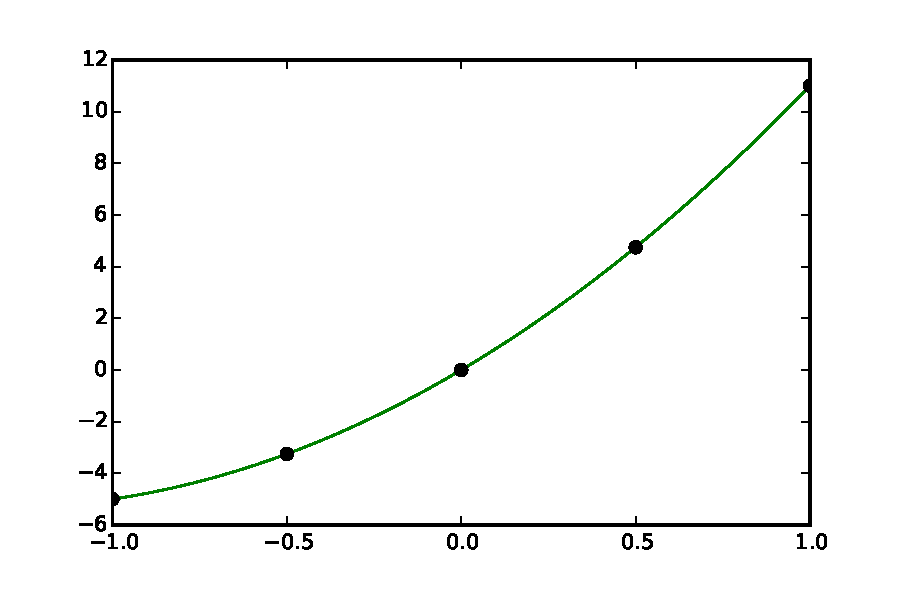
\includegraphics[width=\textwidth]{firstder.pdf}
		\caption{Interpolated first order derivative of the function.}
	\end{subfigure}\\

\caption{Lineal interpolation of the function $f(x) = {x^3} + 4{x^2} - 10$.}
\label{fig:first der}
\end{figure}

We now proceed like in the finite element method and use the local first order polynomials shown in \cref{fig:loc-pols} to interpolate the function under study.

\begin{figure}[H]
  \centering
  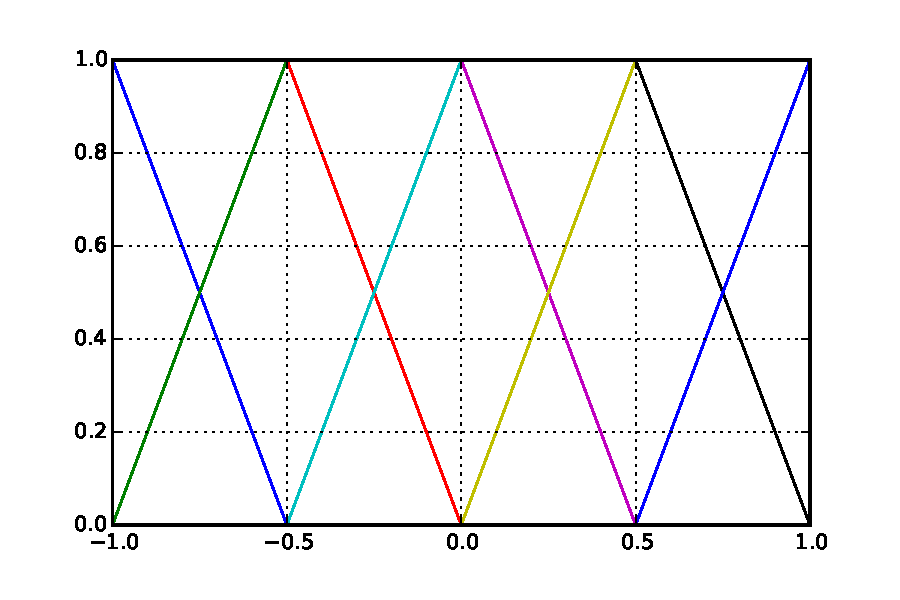
\includegraphics[width=10cm]{localone.pdf}
  \caption{Local interpolating polynomials}
  \label{fig:loc-pols}
\end{figure}

The resulting function and its numerically obtained first order derivateive are shown in \cref{fig:fully local}. It is clear how the local interpolation destroys the global continuity in the first order derivative while the function itself remains continous.


\begin{figure}[H]
\centering
	\begin{subfigure}[b]{0.45\textwidth}\qquad
		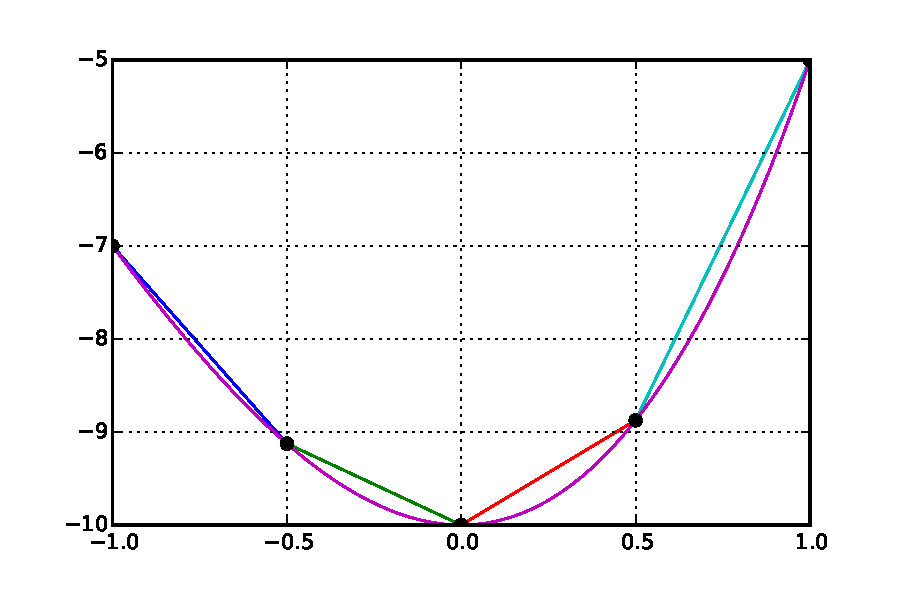
\includegraphics[width=\textwidth]{localfun.pdf}
		\caption{Function interpolated with local first order polynomials. }
	\end{subfigure}\,
%
	\begin{subfigure}[b]{0.45\textwidth}\qquad
		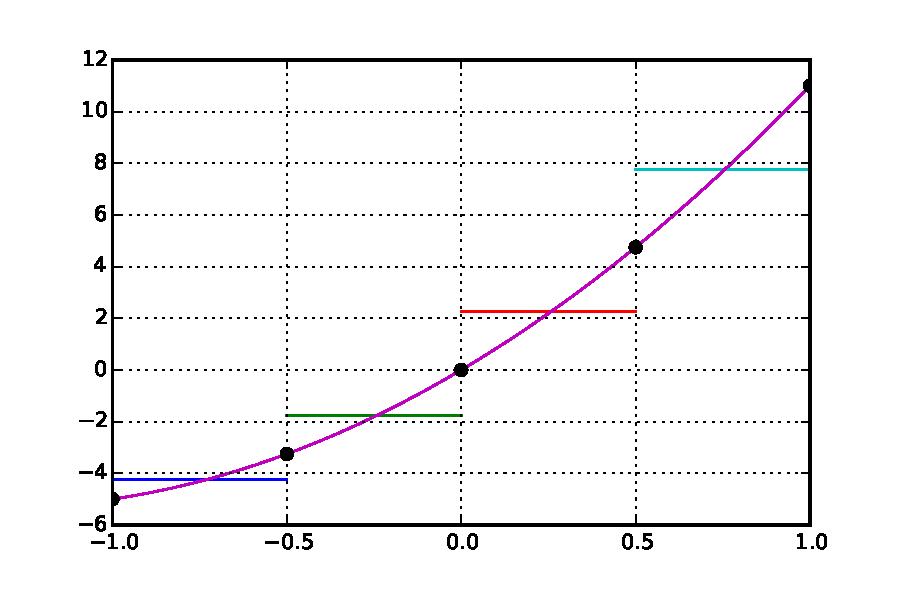
\includegraphics[width=\textwidth]{localfirst.pdf}
		\caption{Interpolated first order derivative of the function.}
	\end{subfigure}\\

\caption{Lineal interpolation of the function $f(x) = {x^3} + 4{x^2} - 10$.}
\label{fig:fully local}
\end{figure}

\subsection*{Extension to 2D domains}
Assume we are now interested in conducting interpolation of a function over a spatial 2-dimensional domain where every point is specified by a position vector of the form $\vb{x} = x \hat{\imath} + y\hat{\jmath}$. We want to know, via interpolation, the value of a function $f(\vb{x})$ at an arbitrary point $\vb{x}$ provided we know the set of n-points $\{(\vb{x}^1, f^1),\cdots,(\vb{x}^n, f^n)\}$.
\begin{figure}[H]\label{fig:element}
  \centering
  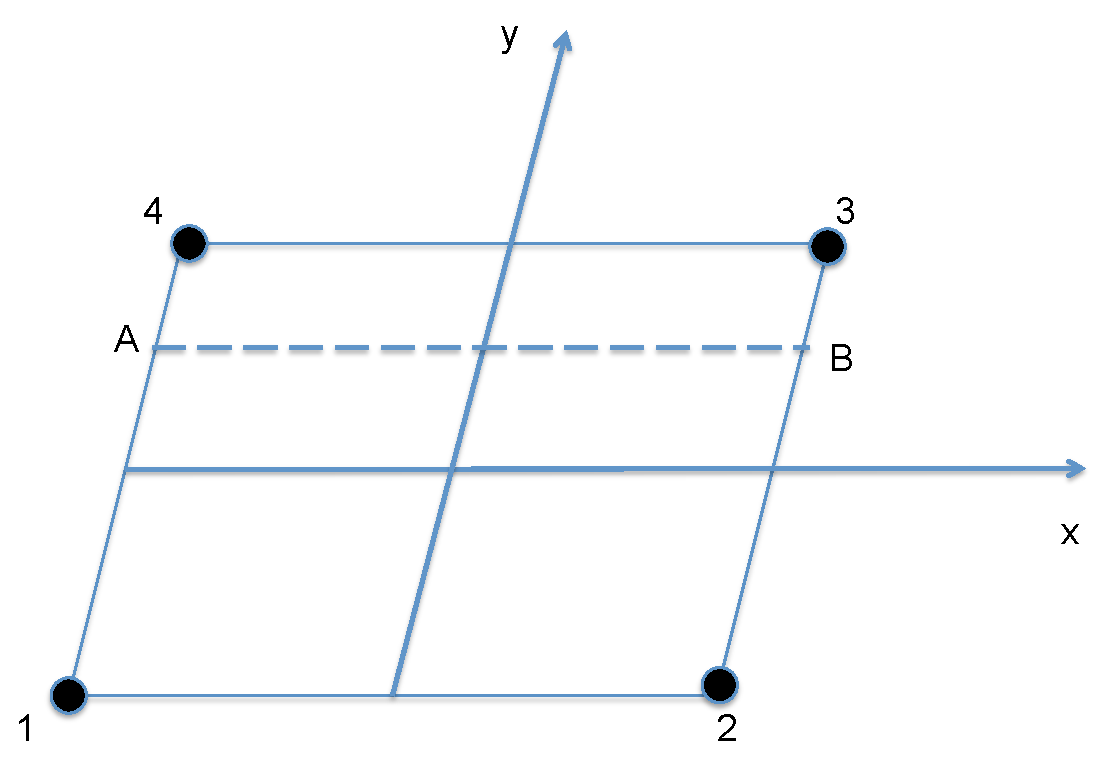
\includegraphics[width=10cm]{element.pdf}
  \caption{Basic square domain}
\end{figure}

We first fix $x = x^A$ and conduct 1-dimensional interpolation along the $y$ direction as discussed in the previous section as follows (see \cref{fig:onedimn})
\[f(x^A,y) = L^1(y)f^1 + L^4(y)f^4\]

\begin{figure}[H]
\centering
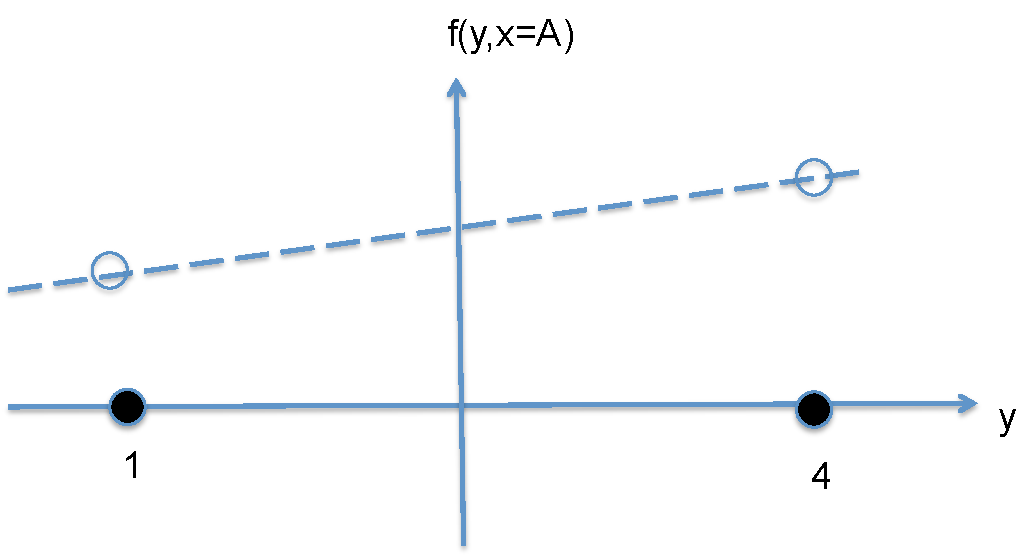
\includegraphics[width=10cm]{inter1D.pdf}
\caption{Interpolation along the $y$-direction}
\label{fig:onedimn}
\end{figure}

Similarly, we can fix $x = x^B$ and interpolate once again along the $y$ direction
\[f(x^B,y) = L^2(y)f^2 + L^3(y)f^3.\]

We now conduct the interpolation along the $x$-direction using the functions $f(x^A,y)$ and $f(x^B,y)$ respectively as follows
\begin{align*}
  &f(x,y) = L^A(x) f(x^A,y) + L^B(x)f(x^B,y)\\
  &f(x,y) = L^A(x)\{L^1(y)f^1 + L^4(y)f^4\} + L^B(x)\{L^2(y)f^2 + L^3(y)f^3\}\\
  &f(x,y) = L^A(x)L^1(y)f^1 + L^A(x)L^4(y)f^4 + L^B(x)L^2(y)f^2 + L^B(x)L^3(y)f^3 \enspace ,
\end{align*}
where
\begin{align*}
L^A(x) & \equiv L^1(x)\\
L^B(x) & \equiv L^2(x)\\
L^1(y) & \equiv L^1(y)\\
L^2(y) & \equiv L^1(y)\\
L^3(y) & \equiv L^2(y)\\
L^4(y) & \equiv L^2(x) \enspace .
\end{align*}

The function of two variables is then written as the product of one-dimensional interpolations
\[f(x,y) = N^1(x,y)f^1 + N^2(x,y)f^2 + N^3(x,y)f^3 + N^4(x,y)f^4\]
with
\begin{align*}
N^1(x,y) & = L^1(x)L^1(y)\\
N^2(x,y) & = L^2(x)L^1(y)\\
N^3(x,y) & = L^2(x)L^2(y)\\
N^4(x,y) & = L^1(x)L^2(y) \enspace .
\end{align*}

See Figure \ref{fig:four-nodes-interp} for the shape functions of a 4-nodes element.
\begin{figure}[H]
\centering
	\begin{subfigure}[b]{0.45\textwidth}\qquad
		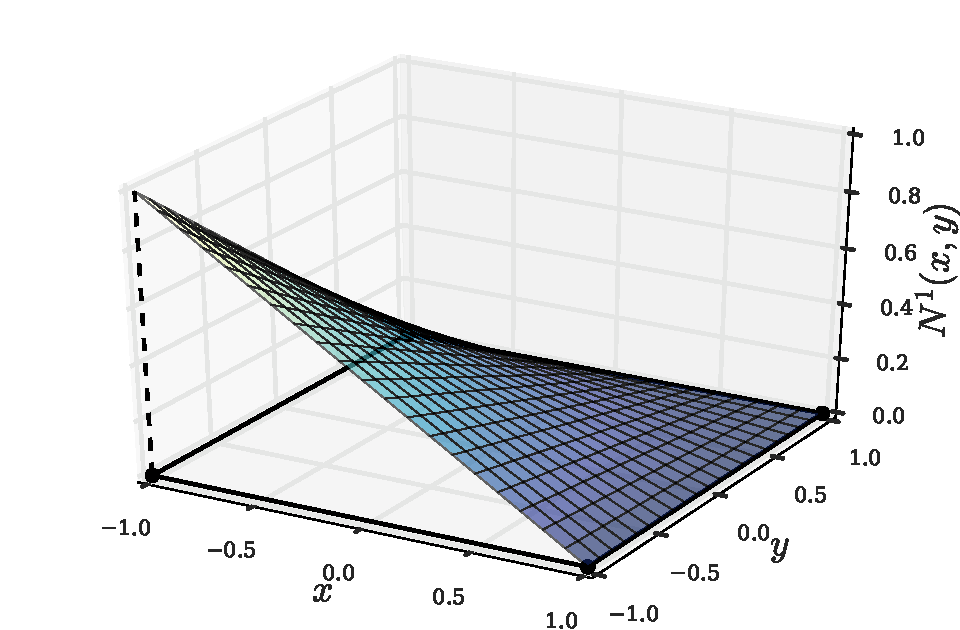
\includegraphics[width=\textwidth]{shape_func-4-nodes-1.pdf}
		\caption{Shape function ${N^1(x,y)=\frac{1}{4}(1-x)(1-y)}$. }
	\end{subfigure}\,
%
	\begin{subfigure}[b]{0.45\textwidth}\qquad
		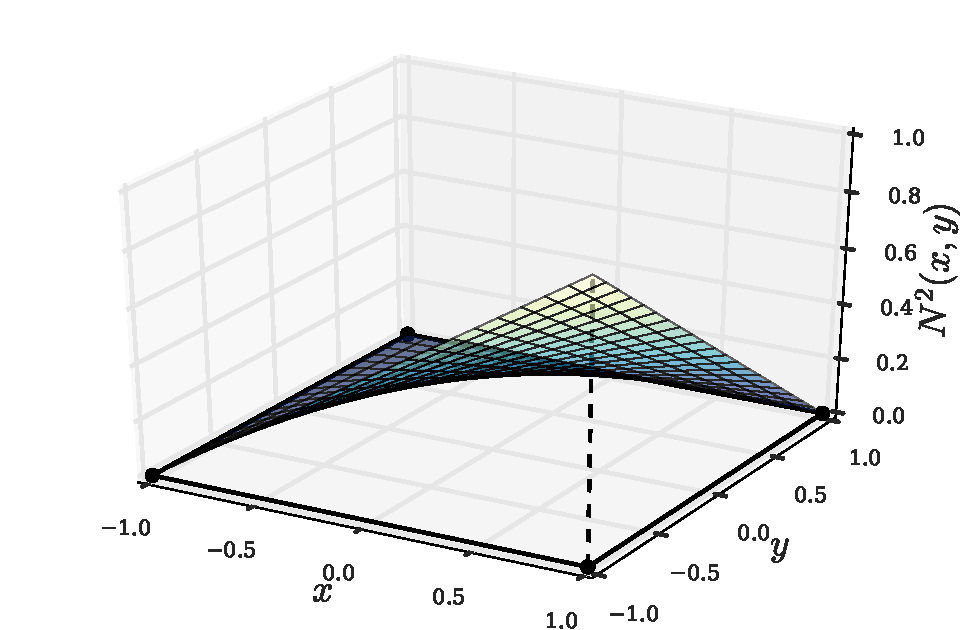
\includegraphics[width=\textwidth]{shape_func-4-nodes-2.pdf}
		\caption{Shape function ${N^2(x,y)=\frac{1}{4}(1+x)(1-y)}$.}
	\end{subfigure}\\
%
	\begin{subfigure}[b]{0.45\textwidth}\qquad
		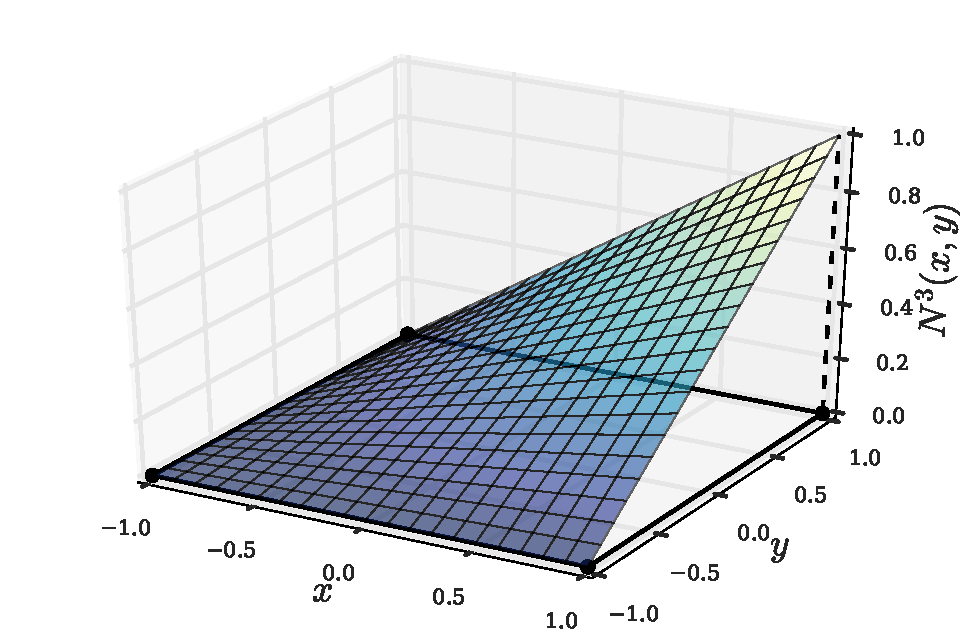
\includegraphics[width=\textwidth]{shape_func-4-nodes-3.pdf}
		\caption{Shape function ${N^3(x,y)=\frac{1}{4}(1+x)(1+y)}$.}
	\end{subfigure}\,
%
	\begin{subfigure}[b]{0.45\textwidth}\qquad
		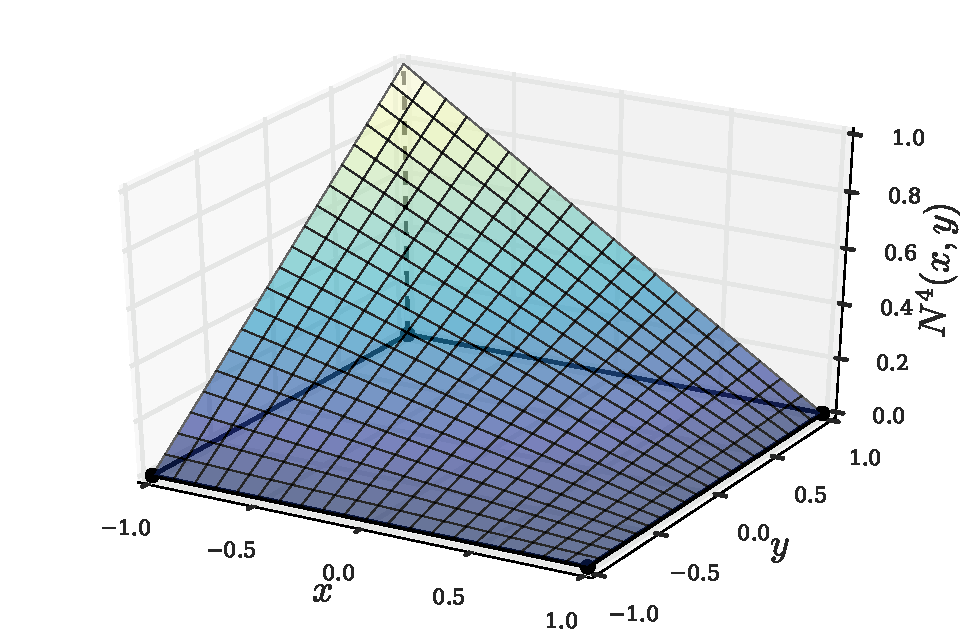
\includegraphics[width=\textwidth]{shape_func-4-nodes-4.pdf}
		\caption{Shape function ${N^4(x,y)=\frac{1}{4}(1-x)(1+y)}$.}
	\end{subfigure}
\caption{Shape functions for a 4-nodes element.}
\label{fig:four-nodes-interp}
\end{figure}

See Figure \ref{fig:nine-nodes-interp} for the shape functions of a 9-nodes element.
\begin{figure}[H]
\centering
	\begin{subfigure}[b]{0.45\textwidth}\qquad
		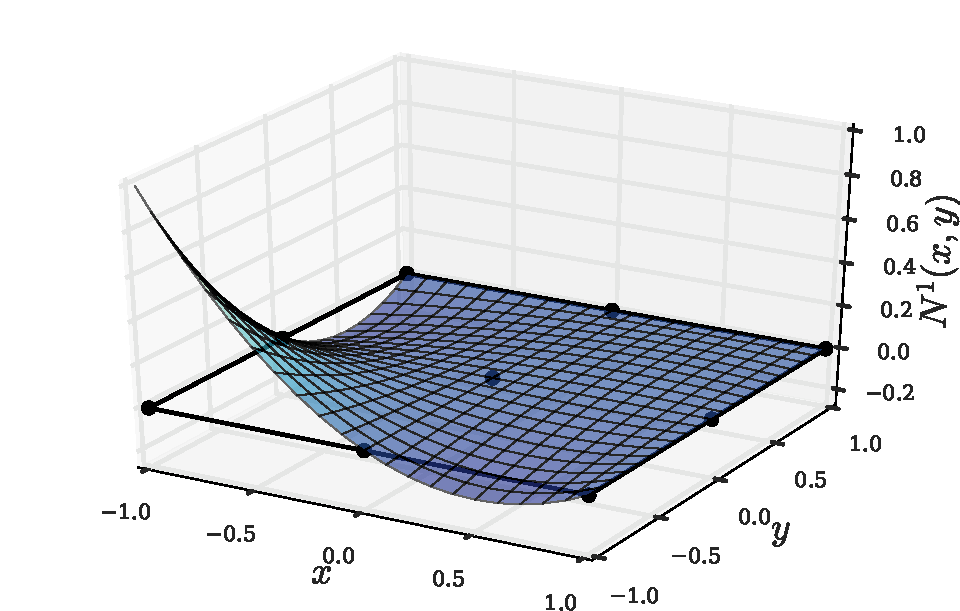
\includegraphics[width=\textwidth]{shape_func-9-nodes-1.pdf}
		\caption{Shape function $N^1(x,y)$. }
	\end{subfigure}\,
%
	\begin{subfigure}[b]{0.45\textwidth}\qquad
		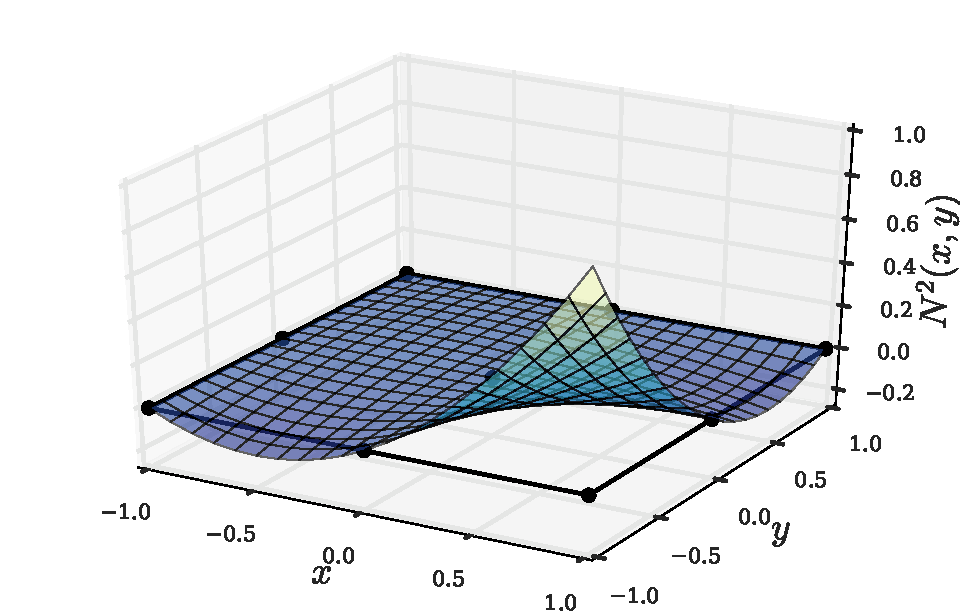
\includegraphics[width=\textwidth]{shape_func-9-nodes-2.pdf}
		\caption{Shape function $N^2(x,y)$.}
	\end{subfigure}\\
%
	\begin{subfigure}[b]{0.45\textwidth}\qquad
		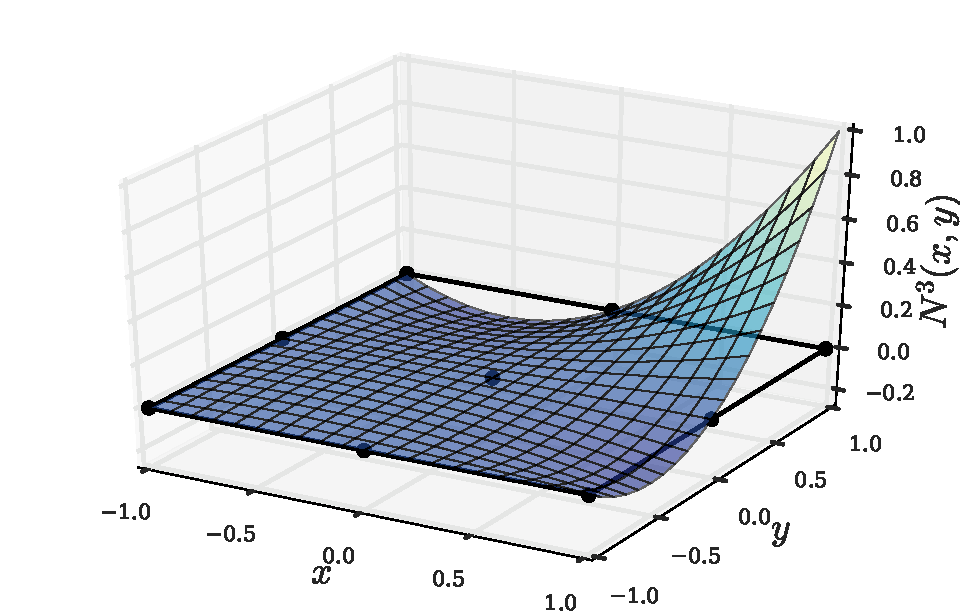
\includegraphics[width=\textwidth]{shape_func-9-nodes-3.pdf}
		\caption{Shape function $N^3(x,y)$.}
	\end{subfigure}\,
%
	\begin{subfigure}[b]{0.45\textwidth}\qquad
		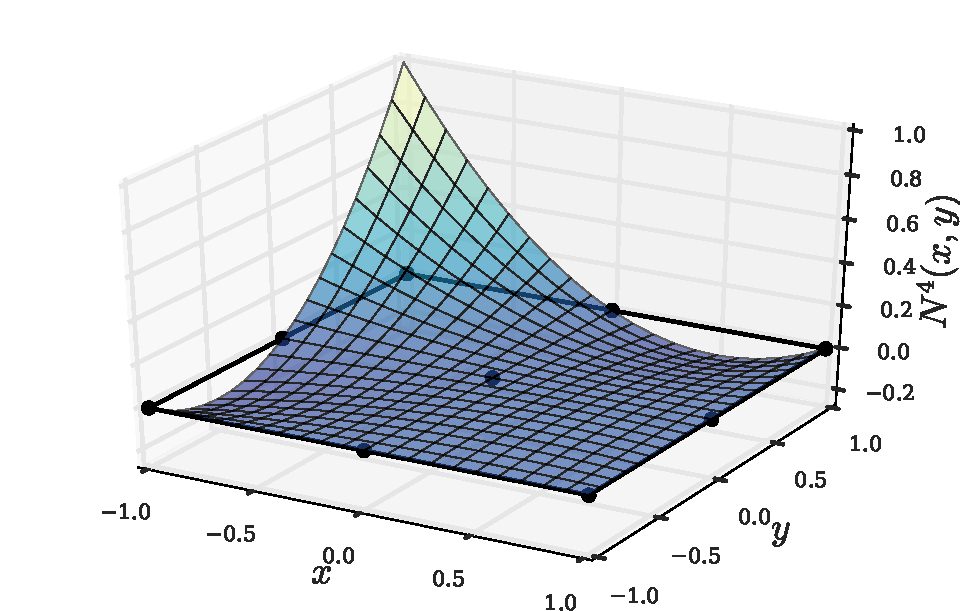
\includegraphics[width=\textwidth]{shape_func-9-nodes-4.pdf}
		\caption{Shape function $N^4(x,y)$.}
	\end{subfigure}\\
	%
	\begin{subfigure}[b]{0.45\textwidth}\qquad
		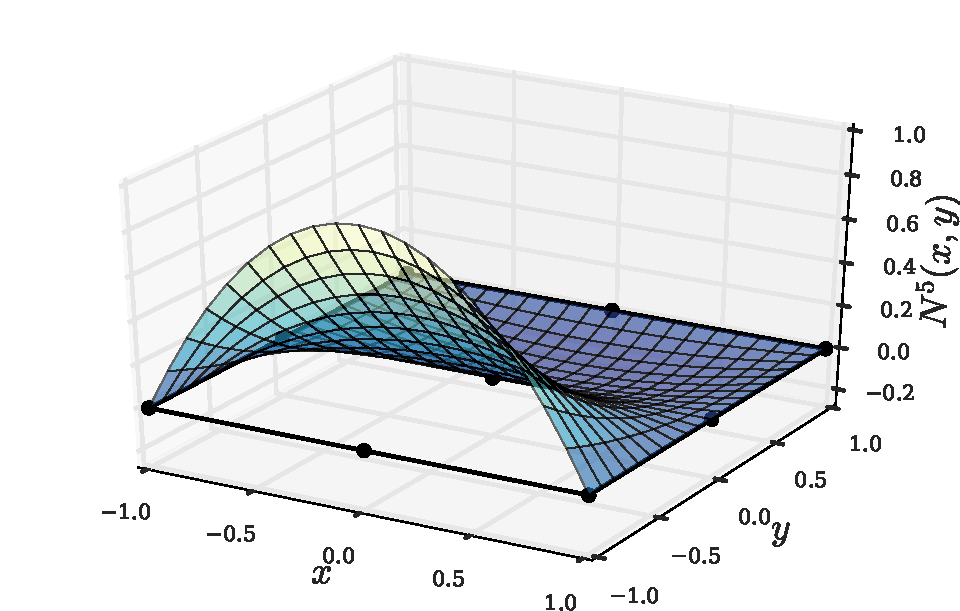
\includegraphics[width=\textwidth]{shape_func-9-nodes-5.pdf}
		\caption{Shape function $N^5(x,y)$.}
	\end{subfigure}\,
%
	\begin{subfigure}[b]{0.45\textwidth}\qquad
		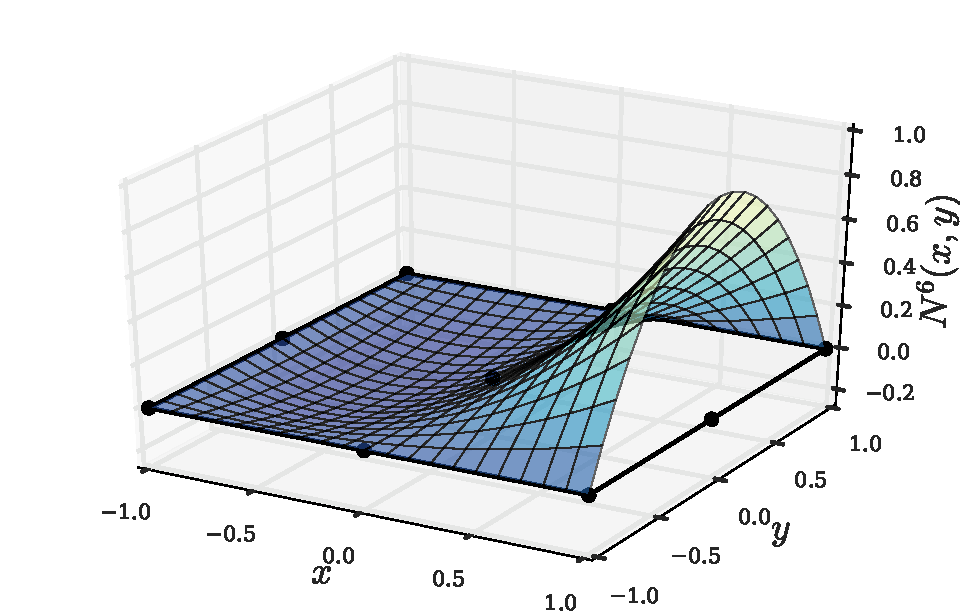
\includegraphics[width=\textwidth]{shape_func-9-nodes-6.pdf}
		\caption{Shape function $N^6(x,y)$.}
	\end{subfigure}
	\caption{Shape functions for a 9-nodes element.}
	\label{fig:nine-nodes-interp}
\end{figure}
%
\begin{figure} [H]
	\ContinuedFloat
	\centering
	\begin{subfigure}[b]{0.45\textwidth}\qquad
		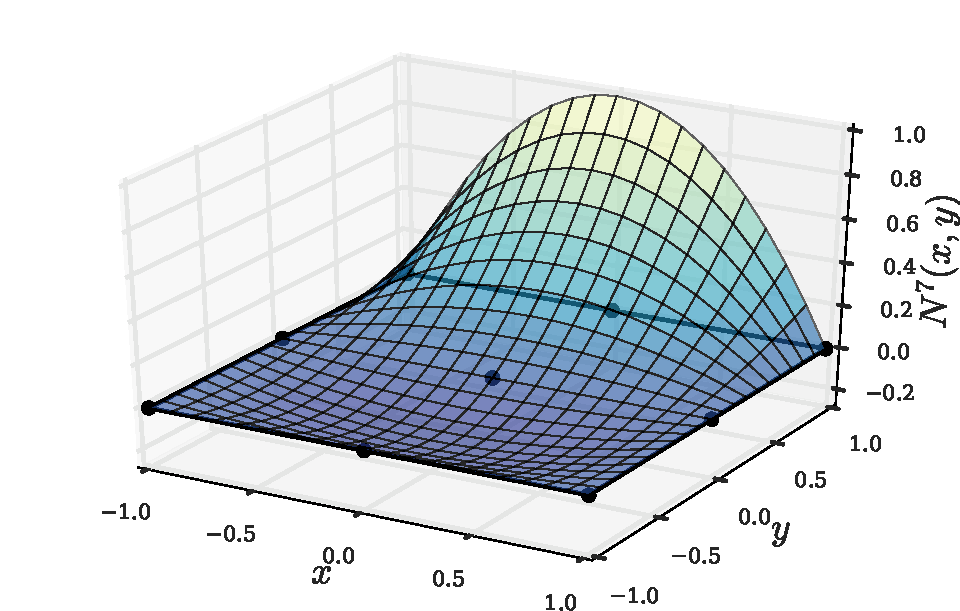
\includegraphics[width=\textwidth]{shape_func-9-nodes-7.pdf}
		\caption{Shape function $N^7(x,y)$.}
	\end{subfigure}\,
%
	\begin{subfigure}[b]{0.45\textwidth}\qquad
		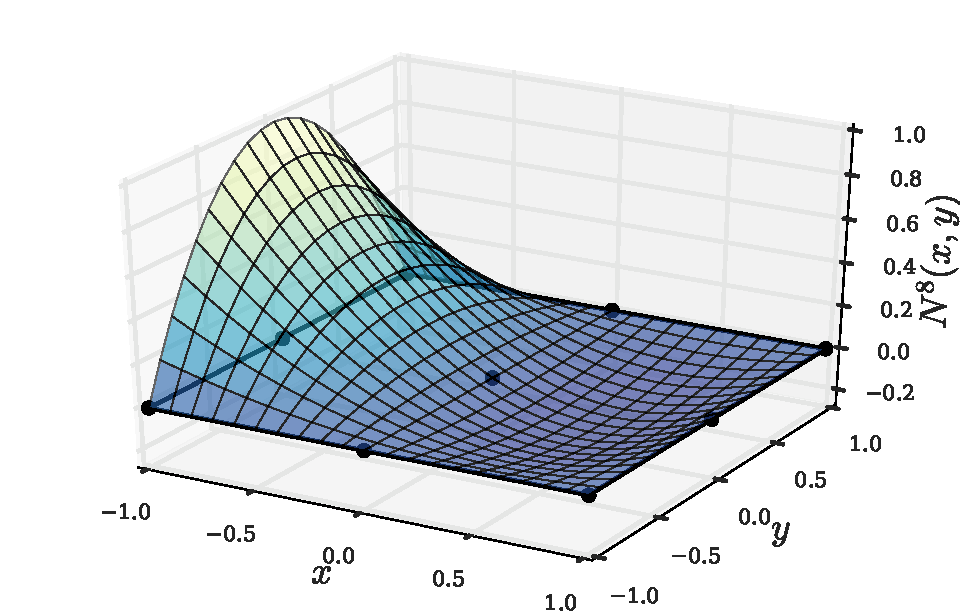
\includegraphics[width=\textwidth]{shape_func-9-nodes-8.pdf}
		\caption{Shape function $N^8(x,y)$.}
	\end{subfigure}\\
	%
	\begin{subfigure}[b]{0.45\textwidth}\qquad
		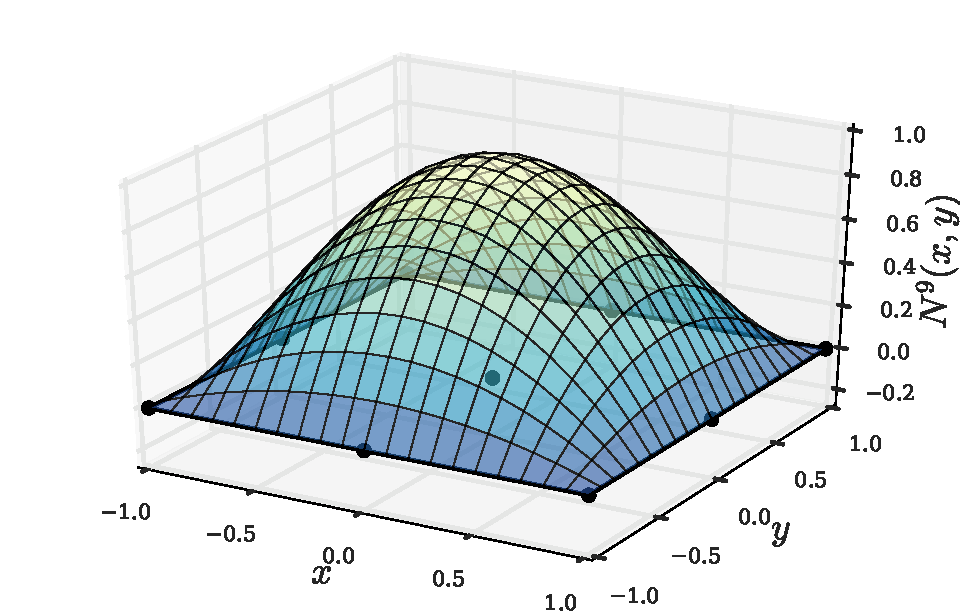
\includegraphics[width=\textwidth]{shape_func-9-nodes-9.pdf}
		\caption{Shape function $N^9(x,y)$.}
	\end{subfigure}
\caption{Shape functions for a 9-nodes element. (Continued)}
\end{figure}

\subsection{Formulation of the finite element matrices}
We now discretize the principle of virtual work repeated below for completeness:
\begin{equation} \label{pvw_2}
\intL_V \sigma_{ij} \delta u_{i,j} \dd{V} - \intL_V f_i \delta u_i \dd{V} - \intL_{S_t} t_i^n \delta u_i \dd{S} = 0.
\end{equation}

For that purpose we will divide the complete domain $V$ into $N$-finite non-overlapping sub-domains over each one of which we will approximate the solution in terms of local interpolating functions (see \cref{fig:fully local}). Since the PVW (or weak form of the BVP) has been cast into an integral representation, it is possible to build the total integral considering the contribution of the $N$-sub-domains like:
\begin{equation}\label{pvw_dis}
\sum_{e=1}^{NEL} \intL_{V^e} \sigma_{ij} \var{u}_{i,j} \dd{V^e} - \intL_V f_i \var{u}_i \dd{V^e} - \intL_{S_t} t_i^n \var{u}_i\dd{S^e} = 0 
\end{equation}

For simplicity we consider only a single element or sub-domain, thus;

\begin{equation}\label{pvw_sing}
\intL_V \sigma_{ij} \delta\epsilon_{i,j} dV - \intL_V f_i\delta u_idV - \intL_{S_t} t_i^n \delta u_i dS = 0
\end{equation}

where it is assumed that the discretized version of each element is later added up (or assembled) into the global equations for the complete model and where we have already used the fact that $\sigma_{ij}$ is symmetric impliying that $\sigma_{ij} \delta u_{i,j} = \sigma_{ij} \delta\epsilon_{i,j}$.

The involved functions (e.g., displacements, strain, stresses) will be approximated via interpolation of the solution over a determined number of points termed in what follows nodes. Assume for instance that over element $e$ containing $n$ such nodes we know the displacements vector $u_i$. For instance, \cref{fig:simple element} below shows a typical square 4-noded element of side $2h$. The rectangular components of the displacement vector at each node are labeled like $[u_1, u_2,...,u_7, u_8]$.

\begin{figure}[H]
\centering
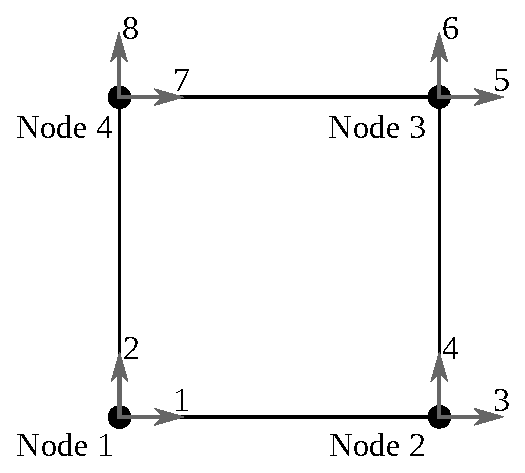
\includegraphics[width=7cm]{lado2h.pdf}
\caption{Square element of side $2h$.}
\label{fig:simple element}
\end{figure}


Furthermore, in a more general treatment, we let the displacements for an arbitrary $p$-node of a $3D$ problem $u^P=[u^P, v^P, w^P]$. Using ideas from interpolation theory it is now possible to approximate the displacements vector over an arbitrary point $\vb{x}$ inside the element by;

\[u_i(\vb x) = N_i^1(\vb x)u^1 + N_i^2(\vb x)u^2 + \cdots + N_i^P(\vb x)u^P + \cdots + N_i^n(\vb x)u^n\]

or in more general form

\begin{equation} \label{bas_interpol}
{u_i}(\vb x) = N_i^Q(\vb x){u^Q}
\end{equation}

and where the caption superscripts indicate summation over the number of nodes of the element while the subscript refers to the physical character of the variable being interpolated.

Now let us use the kinematic relationshio between strains and displpacements:

\[ \varepsilon_{ij}(\vb x) = \frac{1}{2}( u_{i,j} + u_{j,i} ) \]

together with \cref{bas_interpol}. Carrying the derivatives into the shape functions yields;

\[ \varepsilon_{ij}(\vb x) = \frac{1}{2}\left(\pdv{N_i^Q}{x_j} + \pdv{N_j^Q}{x_i} \right){u^Q} \]

which can be written like

\begin{equation}
\varepsilon_{ij}(\vb x) = B_{ij}^Q(\vb x){u^Q}
\label{str-dis}
\end{equation}

after letting

\[ B_{ij}^Q = \frac{1}{2}\left(\pdv{N_i^Q}{x_j} + \pdv{N_j^Q}{x_i} \right). \]

Proceeding analogously for the virtual fields after using

\[ \delta {u_i} = N_i^Q(\vb x)\delta {u^Q} \] gives us:



\[ \intL_V C_{ijkl} B_{kl}^P u^P B_{ij}^Q\delta u^Q \dd{V} - \intL_V f_i N_i^Q\delta {u^Q}\dd{V}  - \intL_{S_t} t_i^n N_i^Q\delta {u^Q} \dd{S} = 0 \]



which can be re-organized into;

\[ \delta {u^Q}\intL_V B_{ij}^Q C_{ijkl} B_{kl}^P\dd{V}{u^P} - \delta {u^Q}\intL_V N_i^Q{f_i}\dd{V}  - \delta {u^Q}\intL_{S_t} N_i^Qt_i^n\dd{S} = 0\]





which is the generalized discrete version of the PVW for a single element consistent with \cref{pvw_sing}. Defining the terms corresponding to the integrals like:


\begin{equation}
\begin{aligned}
{K^{QP}} & = \int\limits_V {{C_{ijkl}}B_{kl}^PB_{ij}^QdV} \\
f_c^Q    & = \int\limits_S {N_i^Qt_i^ndS} \\
f_V^Q    & = \int\limits_V {N_i^Q{f_i}dV}
\label{Rigi_3}
\end{aligned}
\end{equation}


%\begin{align*}
%{K^{QP}} & = \int\limits_V {{C_{ijkl}}B_{kl}^PB_{ij}^QdV} \\
%f_c^Q    & = \int\limits_S {N_i^Qt_i^ndS} \\
%f_V^Q    & = \int\limits_V {N_i^Q{f_i}dV}
%\end{align*}

allows us to write:


\[ \delta u^Q f_\sigma ^Q - \delta {u^Q}f_V^Q - \delta u^Q f_c^Q = 0. \]

This equation is once again the generalized discrete version of the PVW corresponding to the $Q$-displacement degree of freedom. The equation quantifies the work of the forces along the $Q$-th degree of freedom over the virtual displacements $\delta u^Q$. If we now use the arbitrary character of the virtual field $\delta u^Q $ we can write;

\begin{equation}
f_\sigma ^Q - f_V^Q - f_c^Q = 0.
\label{forces}
\end{equation}

This is now a mechanical equilibrium equation relating the forces along the $Q$-th degree of freedom associated to the internal element stresses $f_\sigma ^Q$; the external body forces $f_V^Q$ and the applied external tractions $f_c^Q$. Introducing the stiffness of the element gives:

\begin{equation}
K^{QP} u^P = f_V^Q + f_c^Q.
\label{Discreta}
\end{equation}

\subsubsection{Formulation for square elements}
In the previous section we recognized:

\begin{equation}
\begin{aligned}
{K^{QP}} & = \int\limits_V {{C_{ijkl}}B_{kl}^PB_{ij}^QdV} \\
f_c^Q    & = \int\limits_S {N_i^Qt_i^ndS} \\
f_V^Q    & = \int\limits_V {N_i^Q{f_i}dV}
\label{Rigi}
\end{aligned}
\end{equation}



as the elemental stiffness matrix and the vectors of consistent contact and body forces for a single element. Let us assume that the domain of the single element is a perfect square of side $2h$ (see \cref{fig:lado2h}), thus;

\begin{equation}
\begin{aligned}
K & = \int\limits_{ - h}^{ + h} {\int\limits_{ - h}^{ + h} {{B^T}CBdxdy} } \\
{f_c} & = \int\limits_{ - h}^{ + h} {{N^T}{t^n}ds} \\
{f_v} & = \int\limits_{ - h}^{ + h} {\int\limits_{ - h}^{ + h} {{N^T}fdxdy} }
\label{ele2}
\end{aligned}
\end{equation}

\begin{figure}[H]
\centering
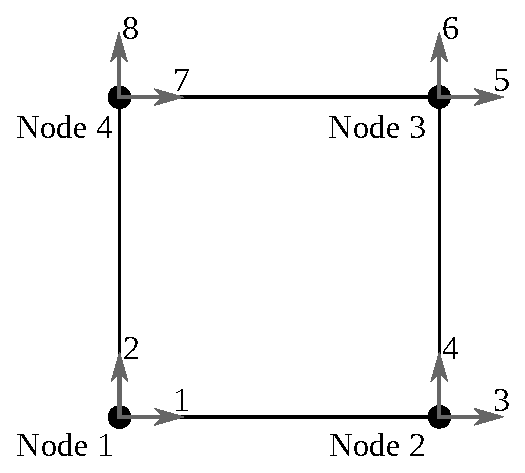
\includegraphics[width=7cm]{lado2h.pdf}
\caption{Square element of side $2h$.}
\label{fig:lado2h}
\end{figure}


and where $N$ and $B$ are the displacements interpolation matrix and the strain-displacements interpolation matrix respectively. For the linear 4-noded element shown in \cref{fig:lado2h} these matrices have the form defined in the following interpolation equations:


\[\left\{ {\begin{array}{*{20}{c}}
{u(\vec x)}\\
{v(\vec x)}
\end{array}} \right\} = \left[ {\begin{array}{*{20}{c}}
{{N^1}(\vec x)}&0&{{N^2}(\vec x)}&0&{{N^3}(\vec x)}&0&{{N^4}(\vec x)}&0\\
0&{{N^1}(\vec x)}&0&{{N^2}(\vec x)}&0&{{N^3}(\vec x)}&0&{{N^4}(\vec x)}
\end{array}} \right]\left\{ {\begin{array}{*{20}{c}}
{{u^1}}\\
{{u^2}}\\
{{u^3}}\\
{{u^4}}\\
{{u^5}}\\
{{u^6}}\\
{{u^7}}\\
{{u^8}}
\end{array}} \right\}\]


\[\left\{ {\begin{array}{*{20}{c}}
{\frac{{\partial u}}{{\partial x}}}\\
{\frac{{\partial v}}{{\partial y}}}\\
{\frac{{\partial v}}{{\partial x}} + \frac{{\partial u}}{{\partial y}}}
\end{array}} \right\} = \left[ {\begin{array}{*{20}{c}}
{\frac{{\partial {N^1}(\vec x)}}{{\partial x}}}&0&{\frac{{\partial {N^2}(\vec x)}}{{\partial x}}}&0&{\frac{{\partial {N^3}(\vec x)}}{{\partial x}}}&0&{\frac{{\partial {N^4}(\vec x)}}{{\partial x}}}&0\\
0&{\frac{{\partial {N^1}(\vec x)}}{{\partial y}}}&0&{\frac{{\partial {N^2}(\vec x)}}{{\partial y}}}&0&{\frac{{\partial {N^3}(\vec x)}}{{\partial x}}}&0&{\frac{{\partial {N^4}(\vec x)}}{{\partial x}}}\\
{\frac{{\partial {N^1}(\vec x)}}{{\partial x}}}&{\frac{{\partial {N^1}(\vec x)}}{{\partial y}}}&{\frac{{\partial {N^2}(\vec x)}}{{\partial x}}}&{\frac{{\partial {N^2}(\vec x)}}{{\partial y}}}&{\frac{{\partial {N^3}(\vec x)}}{{\partial x}}}&{\frac{{\partial {N^3}(\vec x)}}{{\partial y}}}&{\frac{{\partial {N^4}(\vec x)}}{{\partial x}}}&{\frac{{\partial {N^4}(\vec x)}}{{\partial y}}}
\end{array}} \right]\left\{ {\begin{array}{*{20}{c}}
{{u^1}}\\
{{u^2}}\\
{{u^3}}\\
{{u^4}}\\
{{u^5}}\\
{{u^6}}\\
{{u^7}}\\
{{u^8}}
\end{array}} \right\}\]

with the independent shape functions being:


\begin{align*}
{N^1}(x) & = \frac{1}{4}(1 - x)(1 - y) \\
{N^2}(x) & = \frac{1}{4}(1 + x)(1 - y) \\
{N^3}(x) & = \frac{1}{4}(1 + x)(1 + y) \\
{N^4}(x) & = \frac{1}{4}(1 - x)(1 + y)
\end{align*}




Notice that in the computation of the stiffness matrix we actually require the spatial derivatives of the shape functions given by;

\begin{align*}
\frac{{\partial {N^1}(x)}}{{\partial x}} & =  - \frac{1}{4}(1 - y)           &  \frac{{\partial {N^1}(x)}}{{\partial y}} & =  - \frac{1}{4}(1 - x)\\
\frac{{\partial {N^2}(x)}}{{\partial x}} & =  + \frac{1}{4}(1 - y)           &  \frac{{\partial {N^2}(x)}}{{\partial y}} & =  - \frac{1}{4}(1 + x)\\
\frac{{\partial {N^3}(x)}}{{\partial x}} & =  + \frac{1}{4}(1 + y)           &  \frac{{\partial {N^3}(x)}}{{\partial y}} & =  + \frac{1}{4}(1 + x)\\
\frac{{\partial {N^4}(x)}}{{\partial x}} & =  - \frac{1}{4}(1 + y)           &  \frac{{\partial {N^4}(x)}}{{\partial y}} & =  + \frac{1}{4}(1 - y)
\end{align*}


The contribution to the element matrix from a typical nodal point is thus given by;



\[K = \int\limits_{ - h}^{ + h} {\int\limits_{ - h}^{ + a} {\begin{bmatrix}

 \vdots &  \vdots & \vdots &  \vdots & \vdots & \vdots \\
 \cdots &  \frac{{\partial {N^K}(x)}}{{\partial x}} & 0   & \frac{{\partial {N^K}(x)}}{{\partial y}} &  \cdots & \cdots \\
  \cdots &  0 & \frac{{\partial {N^K}(x)}}{{\partial y}}   & \frac{{\partial {N^K}(x)}}{{\partial x}} &  \cdots & \cdots \\
 \vdots &  \vdots & \vdots &  \vdots & \vdots & \vdots 

\end{bmatrix}
%
\begin{bmatrix}
 A & B &  0\\
 B & A & 0 \\
 0 &  0 & C
\end{bmatrix}
%
\begin{bmatrix}
 \cdots & \frac{{\partial {N^Q}(x)}}{{\partial x}} & 0  & \cdots \\
 \cdots & 0 & \frac{{\partial {N^Q}(x)}}{{\partial y}}  & \cdots \\
 \cdots & \frac{{\partial {N^Q}(x)}}{{\partial y}} & \frac{{\partial {N^Q}(x)}}{{\partial x}}  & \cdots 
\end{bmatrix} dxdy} } \]


while a typical element of the resultant stiffness matrix takes the general form:

\[K \equiv A\int\limits_{ - h}^{ + h} {\int\limits_{ - h}^{ + h} {\frac{{\partial {N^K}}}{{\partial x}}\frac{{\partial {N^Q}}}{{\partial x}}dxdy} }  + C\int\limits_{ - h}^{ + h} {\int\limits_{ - h}^{ + h} {\frac{{\partial {N^K}}}{{\partial y}}\frac{{\partial {N^Q}}}{{\partial x}}dxdy.} } \]

It should be noticed that for the considered perfectly square element the resulting stiffness matrix can be partitioned into factors which depend upon the material properties only and into a single factor which depends on the size $h$. This last contribution can be obtained analytically.

Once the elemental matrices are obtained these are assembled into the final global system of equations. Details of the assembly process are discussed in \autoref{chap: Computational Aspects}. The following Python script computes the stiffness matrix for the 4-noded element.

\inputminted[]{python}{src/stiff_4nodes.py}


\subsubsection{Formulation in the natural space: the continuum mechanics analogy}
In typical finite element equilibrium equations we need to perform integration over the reference element domain $V_0(\vb{x})$ corresponding to originally arbitrarily shaped sub-domains as created during the meshing process.  In order to proceed with this integration it is useful to consider the following continuum mechanics analogy.

First assume that the actual physical domain $V_0(\vb{x})$ is the result of a deformation process imparted upon the natural domain as shown in \cref{fig:natural domain}. In this analogy, the physical domain $V_0(\vb{x})$ is regarded like a ``deformed'' configuration at an imaginary time $t=t$, while the natural ``undeformed'' domain $V(\vb{r})$   is treated like a reference undeformed configurations at time $t=0$. Both configurations are assumed to be connected through a deformation process
\begin{equation}
\begin{aligned}
\vb{X}&=\vb{X}(\vb{r})\\
\vb{r}&=\vb{r}(\vb{X})
\end{aligned}
\label{eq:motion}
\end{equation}
\begin{figure}[h]
\centering
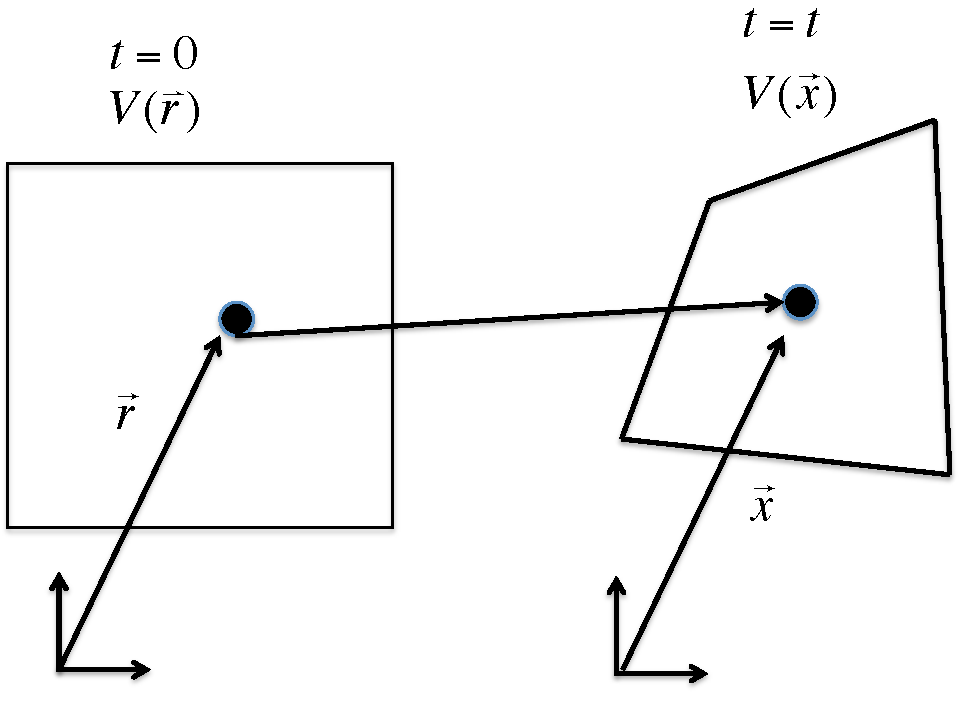
\includegraphics[width=8cm]{figure1.pdf}
\caption{Definition of the natural domain}
\label{fig:natural domain}
\end{figure} 

In \cref{eq:motion} we can understand $\vb{r}$ like a material (Lagrangian) variable and $\vb{X}$ like a spatial (or Eulerian) variable. Using the continuum mechanics analogy it is clear that the ``deformation'' process at the continuum level is fully characterized by the ``deformation'' gradient or Jacobian of the transformation \cref{eq:motion} and defined according to
\begin{equation}
\dd{X}_i=\pdv{X_i}{r_J}\dd{r}_J\equiv J_{iJ}\dd{r}_{J}
\label{eq:gradient}
\end{equation}
where $\dd{r}_{J}$ and $\dd{X}_i$ represent material vectors in the original and deformed configuration. From \cref{eq:gradient} it is evident that the Jacobian contains all the information describing the change of the physical sub-domain with respect to the natural element. For the element integration process we will assume that every element $V(\vb{r})$ in the natural domain deforms into the physical element $V_0(\vb{X})$, thus allowing us to write typical terms like the ones in the material stiffness matrix
\begin{equation}
\intL_{V(\vb{X})} \hat{B}_{ij}^K(\vb{X}) C_{ijkl} \hat{B}_{kl}^P(\vb{X}) dV(\vb{X})\equiv \intL_{V_0(\vb{r})} \hat{B}_{ij}^K(\vb{r}) C_{ijkl} \hat{B}_{kl}^P(\vb{r})J dV_0(\vb{r})
\label{eq:matmatrix}
\end{equation}
where we have used $dV(\vb{X})=JdV(\vb{r})$, with $J$ being the determinant of the deformation gradient and in general we transform functions between the natural and physical space making use of \cref{eq:motion} according to
\begin{equation}
f(\vb{r})=F[\vb{X}(\vb{r})]
\label{eq:funtrans}
\end{equation}


\subsubsection*{Interpolation scheme}
Having identified the fact that the integration process will take place in the natural domain, we will approach the interpolation process directly in this natural space. In the case of the displacement based finite element method all the involved variables will then be obtained via interpolation of nodal displacements. For instance, assume that a given problem variable is defined in the physical space by the tensor $\Phi_{ik...p}(\vb{X})$. The interpolated variable is then written like;

\begin{equation}
\Phi_{ij...p}(\vb{X})=H_{ij...p}^K(\vb{r})\hat{u}^K
\label{eq:interpol}
\end{equation}

where $\hat{u}^K$ represents a vector of nodal points displacements, see \cref{fig:interpol nat dom}, and $H_{ij...p}^K(\vb{r})$ is an interpolator which keeps the tensorial character of the original physical variable $\Phi_{ik...p}(\vb{X})$ and where the super-index makes reference to a nodal identifier (with the summation convention in place).


\begin{figure}[h]
\centering
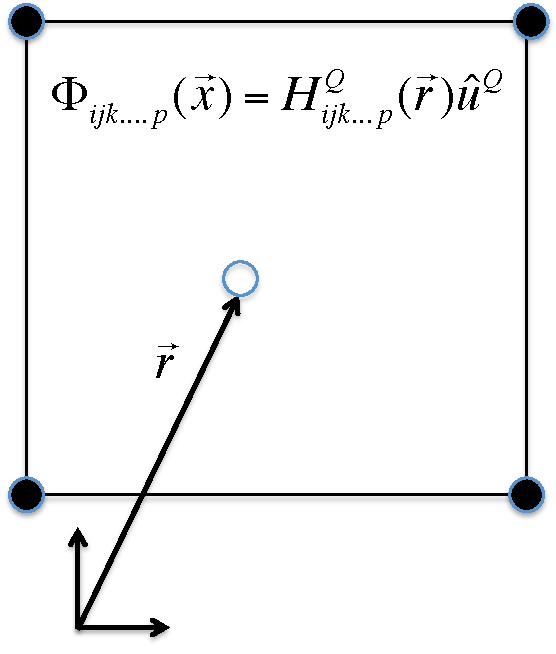
\includegraphics[width=4cm]{figure2.pdf}
\caption{General interpolation strategy in the natural domain}
\label{fig:interpol nat dom}
\end{figure}
 


Since the primary variable corresponds to displacements it must be kept in mind that $H_{ij...p}^K(\vb{r})$ corresponds to combinations of derivatives (or other arbitrary combinations) of the basic element shape functions defined in;


\begin{equation}
u_i(\vb{X})=N_i^K(\vb{r})\hat{u}^K
\label{eq:el interpol}
\end{equation}



For the general interpolation process we need two kinds of transformations.  First we need to transform integrals over the physical space into integrals into the natural space which corresponds to
\begin{equation}
\intL_{V(\vb{X})} F(\vb{X})dV(\vb{X})\equiv \intL_{V_0(\vb{r})} f(\vb{r})J dV_0(\vb{r})
\label{gen trans}
\end{equation}



Second we need to relate spatial differentiation in both, the physical and spatial domains.  Let us define these operators like $\nabla_i^X$ and $\nabla_I^r$ respectively. It then follows from \cref{eq:funtrans} that
\begin{equation}
\dfrac{\partial F}{\partial X_i}=\dfrac{\partial f}{\partial r_J}\dfrac{\partial r_J}{\partial X_i}
\label{eq:chain}
\end{equation}
from where we can establish the connection between the two operators like


\begin{equation}
\nabla_i^X=J_{iJ}^{-1}\nabla_J^r
\label{eq:fundamental}
\end{equation}


\subsubsection*{The fundamental interpolator}
We further define the fundamental interpolator giving rise to gradients of the primary displacement variable in the physical space according to
\begin{equation}
u_{i,j}(\vb{X})=L_{ij}^K(\vb{r})\hat{u}^K
\label{eq:fund operator}
\end{equation}


This fundamental interpolator  $L_{ik}^K(\vb{r})$ is derived after using \cref{eq:el interpol} and \cref{eq:fundamental} in the physical displacement gradient definition as shown next
\begin{align*}
u_{i,j}(\vb{X})&=\nabla_j^X u_i(\vb{X})\\
u_{i,j}(\vb{X})&=\nabla_j^X N_i^K(\vb{r})\hat{u}^K\\
u_{i,j}(\vb{X})&=J_{jQ}^{-1}\nabla_Q^r N_i^K(\vb{r})\hat{u}^K\\
u_{i,j}(\vb{X})&=J_{jQ}^{-1}N_{i,Q}^K(\vb{r})\hat{u}^K
\end{align*}
then
\begin{equation}
L_{ij}^K(\vb{r})=J_{jQ}^{-1}N_{i,Q}^K(\vb{r})
\label{eq:fundamental interpolator}
\end{equation}

\subsubsection*{Elemental stiffness matrix}
The elemental material stiffness matrix computed in the natural domain of \cref{fig:Nat domain} reads

\begin{equation}
K^{KP}=\intL_{V_0(\vb{r})} \hat{B}_{ij}^K(\vb{r}) C_{ijkl} \hat{B}_{kl}^P(\vb{r})J dV_0(\vb{r})\equiv \intL_{r=-1}^{r=+1}\intL_{s=-1}^{s=+1} \hat{B}_{ij}^K(r,s) C_{ijkl} \hat{B}_{kl}^P(r,s)J(r,s) \mathrm{d}r\mathrm{d}s
\label{eq:elematrix}
\end{equation}



\begin{figure}[h]
\centering
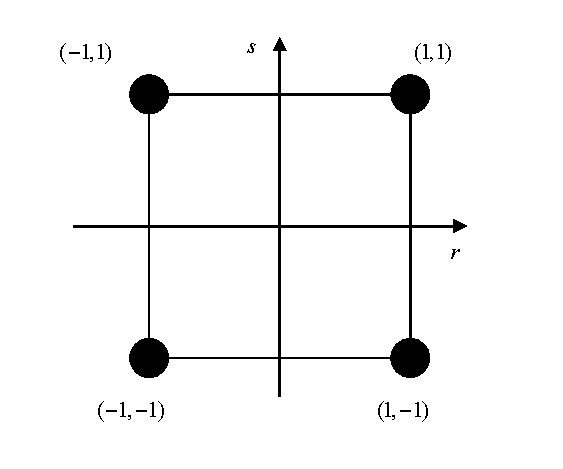
\includegraphics[width=6cm]{figure3.pdf}
\caption{Natural domain of integration}
\label{fig:Nat domain}
\end{figure}
 

Once the interpolator $\hat{B}_{ij}^K(\vb{r})$ has been identified the elemental stiffness matrix is obtained via numerical integration (quadrature) as described in \eqref{eq:eleintegration}

\begin{equation}
\intL_{r=-1}^{r=+1}\intL_{s=-1}^{s=+1} \hat{B}_{ij}^K(r,s) C_{ijkl} \hat{B}_{kl}^P(r,s)J(r,s) \mathrm{d}r\mathrm{d}s\approx \sum_{i,j=1}^\text{NGPTS} \alpha_i \alpha_j \hat{B}_{kl}^K(r_i,s_j)C_{ijkl} \hat{B}_{kl}^P(r_i,s_j) J(r_i,s_j)
\label{eq:eleintegration}
\end{equation}


and where NGPTS corresponds to the number of integration points, $\alpha_j$ is a weighting factor and $r_i,s_j$   are the coordinates of a typical point $\vb{r}$ in the natural space of \cref{fig:Nat domain}.

 
\begin{figure}[h]
\centering
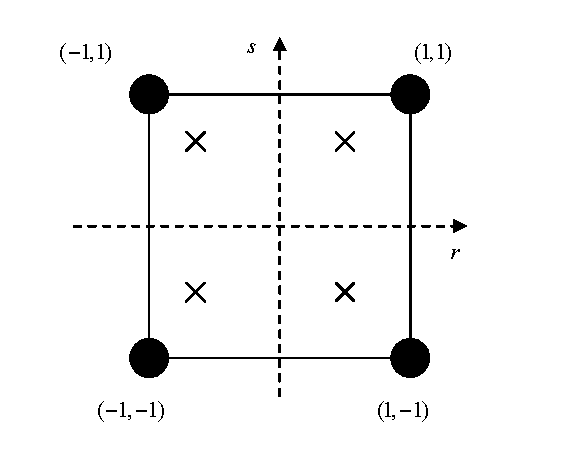
\includegraphics[width=6cm]{figure4.pdf}
\caption{Natural integration domain showing quadrature evaluation nodes}
\label{fig:integration domain}
\end{figure}	 


One important aspect of the numerical integration that has to be kept in mind is accuracy.  Depending on the particularly selected integration scheme, the number of introduced integration points fixes the maximum polynomial order of the considered functions that can be integrated accurately.  In the case of the integrand in \cref{eq:eleintegration}, it is clear that this order increases as the distortion of the physical element  with respect to the natural element increases.  One way of dealing with this dependency of accuracy with element distortion is to make use of adaptative integration techniques which are numerically expensive.  What is actually done in standard FEM analysis is to choose the number of quadrature points beforehand and introduce distortion related error criteria inside the code in such a way that some sort of validation is performed before the numerical integration process is started.

\subsubsection*{Strain displacement interpolator for the infinitesimal strain tensor}
The $Q$-th nodal contribution to the infinitesimal strain-displacement interpolator can be obtained in explicit form as follows. Let $L_x^Q$ and $L_y^Q$ be the spatial differential operators in $x$ and $y$ respectively. We have after expanding \cref{eq:fundamental interpolator}
%
\begin{align*}
L_x^Q & = J_{xP}^{-1}\frac{\partial N^Q}{\partial r_P} \equiv J_{xr}^{-1}\frac{\partial N^Q}{\partial r} + J_{xs}^{-1}\frac{\partial N^Q}{\partial s}\\
L_y^Q & = J_{yP}^{-1}\frac{\partial N^Q}{\partial r_P} \equiv J_{yr}^{-1}\frac{\partial N^Q}{\partial r} + J_{ys}^{-1}\frac{\partial N^Q}{\partial s}
\end{align*}
%
or in matrix form
%
\begin{equation}
\begin{Bmatrix}
L_x^Q\\
L_y^Q
\end{Bmatrix} = 
\begin{bmatrix}
J_{xP}^{-1} &J_{xs}^{- 1}\\
J_{yr}^{-1} &J_{ys}^{- 1}
\end{bmatrix}
\begin{Bmatrix}
\frac{\partial N^Q}{\partial r}\\
\frac{\partial N^Q}{\partial s}
\end{Bmatrix}
\end{equation}

The $Q$-th nodal contribution is then assembled as follows;


\begin{equation}
\begin{Bmatrix}
\pdv{u}{x}\\
\pdv{v}{y}\\
\pdv{u}{y} + \pdv{v}{x}
\end{Bmatrix} =
\begin{bmatrix}
 &L_x^Q &0 \\
\cdots &0 &L_y^Q &\cdots\\
 &L_y^Q &L_{xy}^Q
\end{bmatrix}
\begin{Bmatrix}
\vdots\\
u^Q\\
v^Q\\
\vdots
\end{Bmatrix}
\label{eq:strain inter}
\end{equation}

\begin{algorithm}[H]
    \SetAlgoLined
    \KwData{Nodal coordinates $x^Q$}
    \KwResult{Strain-displacement interpolator $B_{ij}^Q$ }
    Compute Jacobian ${J_{iJ}} = \pdv{N_i^Q}{r_J}{\hat x}^Q$\\
    Invert Jacobian  ${J_{iJ}} \to J_{iJ}^{ - 1}$\\
    Compute fundamental interpolator $L_{ij}^Q = J_{jP}^{ - 1}\pdv{N_i^Q}{r_P}$\\
    Assemble $B_{ij}^Q = \frac{1}{2}\left( {L_{ij}^Q + L_{ji}^Q} \right)$ 
    \caption{Strain-displacement interpolator}
\end{algorithm}



